

\begin{abstract}
There has been a widely documented and recognized increase in diabetes prevalence not only in \acp{HIC} but also in \acp{LMIC}, over recent decades. It is less clear what is the economic burden associated with diabetes, especially in \acp{LMIC}. We provide a systematic review of the global evidence on the costs of type II diabetes. Our review seeks to update and considerably expand the previous major review of the costs of diabetes by capturing the evidence on overall, direct and indirect costs of type II diabetes worldwide that was published since 2001. In addition we include a body of economic evidence that has hitherto been distinct from the \ac{COI} work, i.e. studies on the labour market impact of diabetes. PubMed, EMBASE, EconLit and IBSS were searched (without language restrictions) for studies assessing the economic burden of type 2 diabetes published from January 2001 to October 2014. Costs reported in the included studies were converted to international dollars (\$) adjusted for 2011 values. Alongside the narrative synthesis and methodological review of the studies we conduct an exploratory linear regression analysis, examining the factors behind the considerable heterogeneity in existing cost estimates between and within countries. We identified 86 \ac{COI} and 22 labour market studies. \ac{COI} studies varied considerably in both methods and cost estimates, with most studies not using a control group, though the use of either regression analysis or matching has increased. Direct costs were generally found to be higher than indirect costs. Direct costs ranged from \$242 for a study on \ac{OOP} expenditures in Mexico to \$11917 for a study on the cost of diabetes in the USA, while indirect costs ranged from \$45 for Pakistan to \$16914 for the Bahamas. In \acp{LMIC}---in much contrast to \acp{HIC}---substantial part of the cost burden arose to patients from \ac{OOP} treatment costs. Our regression analysis revealed that direct diabetes costs are closely and positive associated with a country's gross domestic product (GDP) per capita, and that the USA stood out as having particularly high costs, even after controlling for GDP per capita. Studies on the labour market impact of diabetes were almost exclusively confined to \acp{HIC} and found strong adverse effects, particularly for male employment chances. Many of these studies also took into account the possible endogeneity of diabetes, which was not the case for \ac{COI} studies. The reviewed studies indicate a large economic burden of diabetes, most directly affecting patients in \acp{LMIC}. The magnitude of the cost estimates differs considerably between and within countries, calling for the contextualization of the study results. There remains large scope for adding to the evidence base on labour market effects of diabetes in \acp{LMIC}. Further, there is a need for future \ac{COI} studies to incorporate more advanced statistical methods in their analysis to account for possible biases in the estimated costs.

\end{abstract}



\section{Introduction}
Diabetes is a chronic disease that has spread widely, not only in high-income but also in many \acp{LMIC} over the last decades. The most recent data from the International Diabetes Federation indicate that diabetes affected 382 million people worldwide in 2013, a number that is expected to grow to 592 million by 2035. The estimated global prevalence in 2013 amounts to 8.3 \% among people aged 20--79 years, with the world's most populous countries India and China reaching prevalence rates between 9 and 10 \%, corresponding to 65 and 100 million in absolute numbers, respectively. Particularly high prevalence rates are found in Mexico (12.6\%) and Egypt (16.8\%), surpassing the rates of most \acp{HIC}, including the USA (9.2\%) and Germany (8.2\%).\parencite{InternationalDiabetesFederation2013} Taken together, in 2013 about two-thirds of all individuals with diabetes lived in \acp{LMIC} \parencite{InternationalDiabetesFederation2013}. The rising prevalence of diabetes in \acp{LMIC} appears to be fuelled by rapid urbanization, nutrition transition and increasingly sedentary lifestyles \parencite{Hu2011}. The most prevalent form of diabetes by far is type 2 diabetes, affecting about 90 \% of people with diabetes while the remaining 10 \% mainly have type 1 diabetes or gestational diabetes \parencite{InternationalDiabetesFederation2013}.

Due to its adverse effect on people's health diabetes also imposes an economic burden on individuals and households affected as well as on healthcare systems. The economic burden of diabetes was confirmed by   in a review of \ac{COI} studies on diabetes mellitus, published in 2004, covering the literature up to the year 2000. The authors concluded that the direct and indirect economic burden of diabetes was "large", and that costs had increased over time. However, the review also noted that significant variation in costing methodologies made it near impossible to directly compare the cost estimates. However, the studies reviewed by \textcite{Ettaro2004} were almost exclusively focused on the USA, with a small part coming from European \acp{HIC} and none from \acp{LMIC}. The aim of this study is therefore to systematically review the literature on the economic costs of diabetes published since 2001 (i.e. the first year not covered by the \textcite{Ettaro2004} review), as we expect a considerable number of new studies, also from \acp{LMIC}. In addition to the \ac{COI} studies we review the literature on labour market outcomes, with a specific interest in the methodological challenges involved. In doing so we substantively update and expand the scope of the \textcite{Ettaro2004} review, allowing us to revisit its findings regarding the evidence base about the economic burden of type 2 diabetes globally.

\ac{COI} studies generally assess the direct and indirect costs of a particular illness, where the former represent the opportunity cost of resources used for treatment. The indirect costs measure the value of resources lost due the illness, most commonly those caused by losses in productivity due to mortality and morbidity as measured in lost earnings \parencite{Segel2006}. In addition, another approach also focuses on estimating the impact of diabetes on labour market outcomes. However, rather than trying to estimate the monetary losses that arise from a decrease in productivity, these studies typically compare labour market outcomes (e.g. employment probabilities, earnings or lost work days) between people with and without diabetes, while accounting for differences in age, education and other demographic and socioeconomic variables, that might arise between both groups and that could affect labour market outcomes as well as the chances of developing diabetes. The aim of studies in this field is to obtain a clearer picture of how diabetes causally affects these labour market outcomes, without necessarily monetizing the results. Because of the different methodologies and data requirements, these studies tend to differ considerably from traditional \ac{COI} studies, which is why we reviewed them separately. To the best of our knowledge this is the first review that systematically assesses the studies in this particular field.

\section{Methods}

\ac{PRISMA} guidelines were used as a basis for the overall study approach.\parencite{Moher2009b}
\subsection{Search strategy}
The electronic search was based on the following search terms: "Diabetes Mellitus"[Mesh] AND ("Costs and Cost Analysis"[Mesh] OR "Cost of Illness"[Mesh] OR "Employment"[Mesh] OR "Labor Market"[All fields] OR "Labour Market"[All fields] OR "Productivity"OR "Willingness to pay"[All fields]). The above search was run in PubMed and was then adapted for searches in EMBASE, EconLit and the International Bibliography of the Social Sciences (IBSS). The search was carried out from October 2012 to October 2014 and restricted to studies published between January 2001 and October 2014, as the earlier review had covered \ac{COI} studies until 2000 \parencite{Ettaro2004}. No language restrictions were applied. The references were downloaded in RIS format where possible and then transferred to Mendeley. Authors were contacted for further information if clarification was needed after the full text analysis.

\subsection{Inclusion and exclusion criteria}
Studies were eligible if a monetary estimate of the direct and/or indirect costs of diabetes was presented in the results section or if studies provided an estimate of the impact of diabetes on labour market outcomes (employment chances, labour income, wages and lost work days). We did not exclude studies with a small sample size as this might have discriminated against studies in \acp{LMIC}. Studies on types of diabetes explicitly different from type 2 diabetes were excluded. However, we included studies that did not explicitly mention the type of diabetes, given that type 2 diabetes accounts for about 90 \% of all diabetes cases. Studies exclusively assessing the costs of diabetes complications or the costs of management strategies were excluded as were studies estimating the costs for specific groups with diabetes (e.g. costs for people with poorly controlled diabetes), since we were interested in the costs incurred to populations comprising the whole spectrum of people with type 2 diabetes. Editorials, reviews and studies for which the full text could not be retrieved or only an abstract was available were also excluded.

\subsection{Data extraction and analysis}
Data extraction was carried out by two investigators (TS and OA). After duplicates were removed, titles and abstracts were scanned by one researcher (TS) to identify studies suitable for a full text review. The process was checked by a second researcher (OA) on a random subsample of 2000 studies of the retrieved references. The full text was subsequently retrieved for the identified studies and they were reviewed by two researchers (TS and OA), with disagreements resolved by discussion. Finally, 109 studies were identified (see Figure \ref{fig:review_prisma_flowchart}) that fulfilled the inclusion criteria and data extraction was carried out using a pre-defined extraction table. Primary outcomes were the total costs, the direct costs, and the indirect costs of type 2 diabetes and the respective per capita estimates of these outcomes, as well as the impact of type 2 diabetes on employment chances, income, wages and lost work days. Secondary outcomes comprised the methodology used to assess the monetary costs of type 2 diabetes, the range of cost factors included in the analysis, as well as the methodology used to assess the labour market impact of diabetes. Further extracted information included the year of publication, year of data collection, the time horizon, the country or region studied, the data source, sample size and age as well as information on whether the study distinguished between types of diabetes.


\begin{figure}[hp]
\caption{\label{fig:review_prisma_flowchart}\acs*{PRISMA} flowchart.}%
\centering
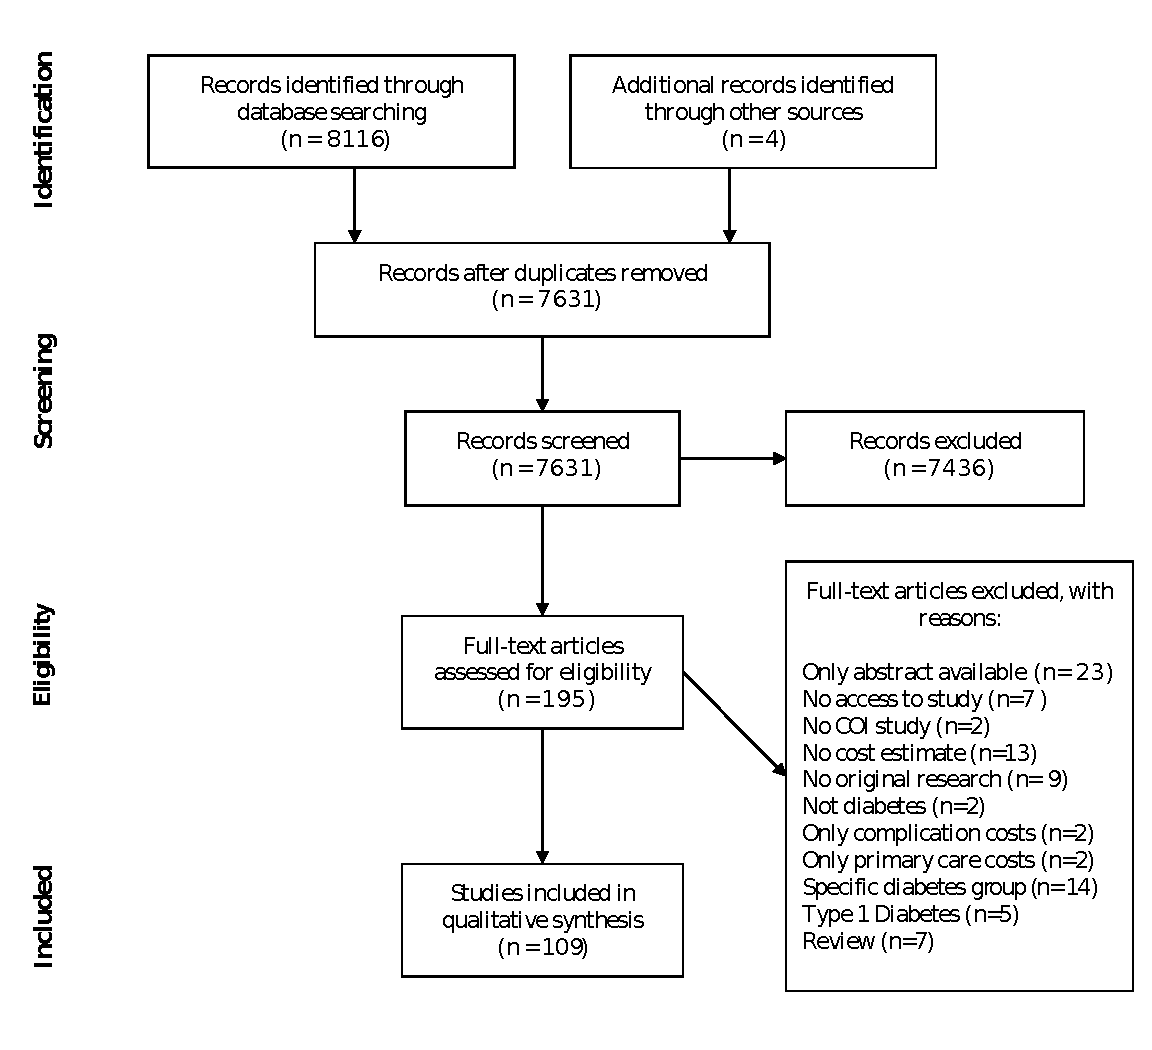
\includegraphics[width=0.9\linewidth]{Review/Figures/Fig1.eps}
\end{figure}

We present the \ac{COI} study results in per capita values to facilitate comparability across countries. For studies presenting overall population level estimates rather than per capita costs information, we calculated those costs, whenever possible, using the diabetes prevalence mentioned in the respective study. If no total cost estimate was presented but information on direct and indirect costs was available, then direct and indirect costs were added up to produce a total cost estimate. We converted costs into \ac{PPP} adjusted estimates, also called international dollars and henceforth denoted with the \$ sign, in order to further increase comparability. Since some studies did not present the data in the country's local currency but in USA\$ or some other major currency, we used the exchange rate given in the article to convert the estimates back into the local currency. If no exchange rate was provided in the study itself, the average exchange rate (midpoint exchange rate according to OANDA historical exchange rates---[\url{http://www.oanda.com/currency/historical-rates/}]) for the reported year. The \ac{PPP} adjusted estimates for the year 2011 were then calculated using the Campbell and Cochrane Economics Methods Group Evidence for Policy and Practice Information and Coordination Centre (CCEMG-EEPPI Centre) cost converter \parencite{Shemilt2010}. For all additional analyses carried out in the following sections only studies for which a mean cost estimate was presented or could be calculated, were included. Further, in the case of a study presenting estimates for more than 1 year, only the estimate for the most recent year was used for the analysis. For studies presenting both incremental and total cost estimates, only the incremental cost estimate was taken into account.

Studies were further classified into two groups according to the level of economic development of the investigated country---(1) high-income and (2) \acp{LMIC} (\acp{LMIC})---according to the historical World Bank income group classification of the respective country in the year that data collection for the respective study had taken place \parencite{WorldBank}. Where necessary due to space constraints we used abbreviations for country names, as detailed in Table \ref{tab:review_countries}.

In order to explore the factors involved in the variation of direct costs reported in \ac{COI} studies, we first plotted the direct per capita costs in relation to the \ac{GDP} per capita of the respective country and provided an estimate of the relationship using linear regression. We then conducted an exploratory regression analysis, with the annual direct cost per patient as the dependent variable to investigate what other factors might explain the variation in direct cost estimates. The set of independent variables comprised (1) the estimation approach in each study, (2) the year of data used, (3) \ac{GDP} per capita of the studied country in international dollars, (4) an indicator of whether the study was conducted in the USA, (5) an indicator of whether the study was deemed to be nationally representative, and (6) a variable indicating whether the study had explicitly taken diabetes-related complications into account. The year of the used data was considered because the development of social security systems and treatment methods may affect how the direct costs evolve over time. We categorized this variable into groups: studies using data from before 1995, 1995 to 1999, 2000 to 2004, 2005--2009 and 2010--2004.  The dummy variable for studies on the USA was included to account for the generally higher healthcare expenditures in the USA compared which other \acp{HIC} with similar per capita income levels \parencite{Laugesen2011}. Accounting for national representativeness should cancel out any effects that might be driven by those studies that estimate costs for sub-national, regional- or city-level population samples. Including an estimator for diabetes complications should account for the possible underestimation of diabetes costs in studies excluding complications. We exclude country estimates extracted from multi-country studies in our preferred specification, as their inclusion would lead to an over-statement of the cost effect of the estimation method employed in the given multi-country study. 

\section{Results}
Due to the differences in methodologies, we first present the findings on the identified \ac{COI} studies and subsequently turn to studies on labour market outcomes.

\subsection{\acs*{COI} studies on type 2 diabetes}

\subsubsection*{Number of studies}
We identified a total of 86 relevant \ac{COI} studies (see Table \ref{tab:COI_charactersitics} for a detailed description of the included studies), of which 62 focused on \acp{HIC}, 23 on \acp{LMIC}, and one multi-country study covered both \acp{HIC} and \acp{LMIC}. Studies in \acp{LMIC} increased over time, with the majority of the \ac{LMIC} studies being published between 2007 and 2014. Six of the selected studies were multi-country studies, of which two \parencite{Kirigia2009,Smith-Spangler2012} did not provide detailed cost estimates for every country in the study and one did not provide a year for the estimated costs, so that we could not calculate estimates in international dollars \parencite{Boutayeb2014}. Therefore, we could not include these particular studies in our country-specific analysis.

\subsubsection*{Regional distribution}
In terms of geographic regions, most studies were carried out on countries in Latin America and the Caribbean (n=38) and Europe (n=37), followed by the USA and Canada (n=26), East Asia and Pacific (n=11), the Middle East and North Africa (n=5), South Asia (n=4), Sub-Saharan Africa (n=4) and Australia (n=1). The number of countries studied is higher than the number of articles reviewed due to four multi-country studies \parencite{Boutayeb2014,Barcelo2003,Jonsson2002b,Abdulkadri2009b}, estimating costs for multiple countries. The USA were the most studied country (n=19), followed by Canada (n=7) and Germany (n=5). Mexico (n=6) and China (n=4) were the most frequently studied \acp{LMIC}.

\subsubsection*{Data sources}
Especially in \acp{LMIC}, self-administered surveys represented a popular method to retrieve data on the cost of diabetes. These were mostly limited regionally, i.e. to a city or hospital, and usually only representative of these regional diabetes populations but not of a national population. In \acp{HIC}, databases of insurance and healthcare providers were the main source of information in most studies. These data tended to be representative either at a national or at some sub-national level. As a result, the size of the samples in \acp{HIC} was mostly between 1,000 and several million. By contrast, studies in low- and lower-middle-income countries were generally characterized by smaller sample sizes, ranging from 35 \parencite{Suleiman2006} to about 2,433 \parencite{Yang2012} in the studies reviewed here.

\subsubsection*{Variation in costing approaches}
As discussed in more detail in Text Box 1, a range of costing approaches can be found in the \ac{COI} literature. Figure \ref{fig:review_COI_number} shows that the most common costing method for the direct costs of diabetes in \acp{HIC} was the sum-all medical approach for people with diabetes without using control groups \parencite{Kirigia2009,Boutayeb2014,Barcelo2003,Jonsson2002b,Ohinmaa2004,Lau2011a,Pohar2007,Gonzalez2009b,Horak2009,Martin2007b,Nolan2006c,Lucioni2003,Morsanutto2006b,Nakamura2008,Arredondo2004,Arredondo2007,Arredondo2005a,Arredondo2011b,Redekop2002b,Bjegovic2007b,Oliva2004a,Ringborg2008a,Chi2011a,Zhou2005a,Condliffe2014,Brandle2003d,Peele2002a,Lee2006,Maciejewski2004}. The disease-attributable costing approach \parencite{Suleiman2006,Abdulkadri2009b,Davis2006b,Simpson2003,RodriguezBolanos2010a,Solli2010a,Ballesta2006,Mata2002a,Lin2004,Dall2003a,Buescher2010,Tunceli2010c,Johnson2006d,Honkasalo2014,Bastida2002} and the attributable-fraction approach were also used widely, though mainly in the USA \parencite{AmericalDiabetesAssociation2008,Dawson2002b,Schmitt-Koopmann2004b,Dall2010,Bolin2009d,Honeycutt2009a,Lesniowska2014}. The incremental cost approach was applied primarily in studies on \acp{HIC} \parencite{Smith-Spangler2012,Yang2012,Tunceli2010c,Honeycutt2009a,Pohar2007a,Ricordeau2003,Koster2011c,Koster2006c,Koster2012,Esteghamati2009,Chodick2005a,Marchesini2011b,Bruno2012,Norlund2001a,Wirehn2008b,Birnbaum2003c,Durden2009b,Rodbard2010b,Oconnell2012,Trogdon2008a,Ramsey2002a,VanderLinden2009c}.  For \acp{LMIC}, the survey approach was the most used \parencite{Wang2009b,Wang2009f,Chan2007a,Ramachandran2007d,Javanbakht2011b,Khowaja2007a,Biorac2009a,Elrayah-Eliadarous2010b,Chatterjee2011c,Al-Maskari2010c,Druss2001,Tharkar2010a,Wang2010c}.


\begin{figure}[hp]
\caption{\label{fig:review_COI_number}Number of \acs*{COI} studies, by costing approach and income group.}%

\begin{minipage}{\linewidth}
\begin{center}
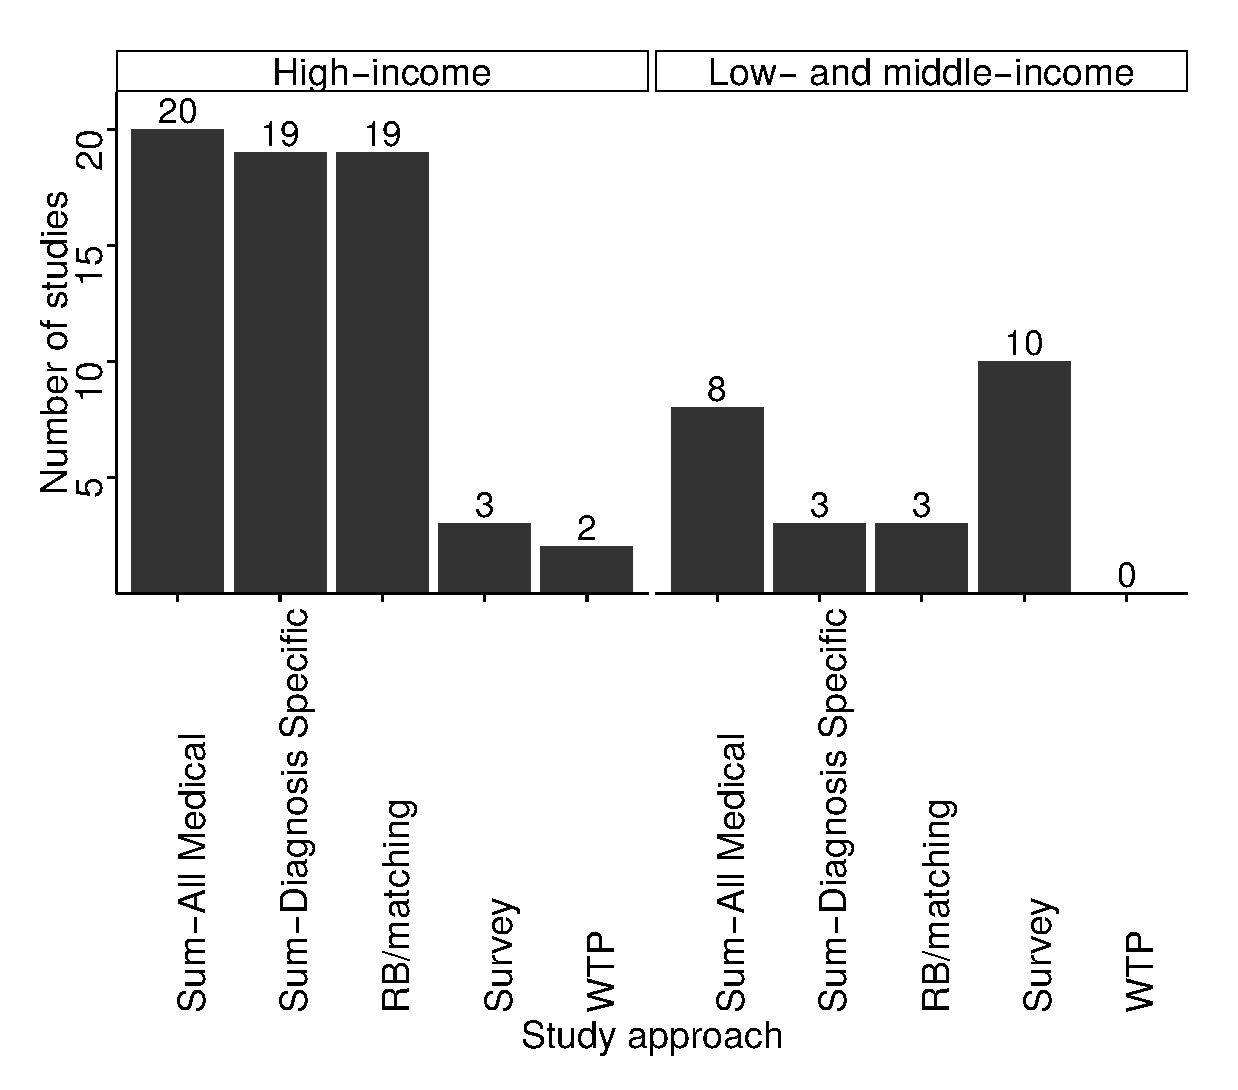
\includegraphics[width=0.8\linewidth]{Review/Figures/Fig2.eps}\\
\end{center}
\footnotesize
\textit{Notes} For \acp{LMIC} no \ac{WTP} study is counted, because the only study \parencite{Tharkar2010a} presenting a \ac{WTP} estimate for a \ac{LMIC} used primarily a different approach to estimate costs, and the \ac{WTP} estimate was only presented additionally. Therefore this study was not counted under \ac{WTP} here. Two studies are counted twice as they give estimates for a sum-diagnosis specific and a RB/matching approach.
\end{minipage}
\end{figure}

By contrast, almost all indirect cost assessments followed the same methodology, i.e. the human capital approach. This approach considers all forgone labour earnings of a patient or caregiver that are attributable to diabetes. A minority of three studies \parencite{Tharkar2010a,Chang2010b,Gyldmark2001}, estimated the indirect costs using the \ac{WTP} approach, which tries to measure how much individuals would be willing to pay to reduce the risk of an illness \parencite{Segel2006}, here diabetes (or certain complications associated with it). One of the studies included \ac{WTP} estimates in addition to the direct and indirect costs measured by the human capital approach \parencite{Tharkar2010a} but did not include the \ac{WTP} estimate in the overall cost estimate, while the other two studies estimated exclusively the \ac{WTP} \parencite{Chang2010b,Gyldmark2001}.

\FloatBarrier

\subsubsection*{Study perspective}
Studies also varied in their perspective, again compromising direct comparability of the cost estimates across studies. Overall, most studies either took a societal (n=32) or healthcare system perspective (n=48). The former generally takes into account the direct and indirect monetary costs that arise to society, including costs to the healthcare system, costs due to lost productivity and sometimes \ac{OOP} costs \parencite{Segel2006}. The latter was especially common in \acp{HIC} where many studies assessed the cost of diabetes to private or public health insurances. In \acp{LMIC}, studies often took the patient perspective (n=5), estimating \ac{OOP} expenditures and in some cases productivity losses, directly arising to the diabetes patient.

%Textbox
\fbox{\parbox[c]{\linewidth}{\textbf{Text box 1 \ac{COI} methodologies}
\begin{footnotesize}

Methodologies for \ac{COI} studies can broadly be categorized into two main categories:(1) estimating the total disease costs and (2) estimating the incremental costs \parencite{Akobundu2006}. Studies can then be divided further according to the specific approach used for estimation. Our categorization builds on that by \textcite{Akobundu2006} in their review of \ac{COI} methodologies.

\begin{enumerate}

\item Total disease costs
\begin{enumerate}
\item Sum-All Medical: captures all medical expenditures of a person diagnosed with diabetes, irrespective of the relation of the expenditures with diabetes.

\item Sum-Diagnosis Specific: includes the costs that are related to diabetes. This can be done by using a disease-attributable costing approach, using administrative claims databases to identify the cost of diabetes by respective \ac{ICD} codes that link the expenditures to a primary or secondary diagnosis of diabetes as the reason for the healthcare utilization. Alternatively, a similar technique used at the population level is the attributable-fraction approach, where the relative contribution of, e.g., diabetes, to the risk of developing another disease (e.g. renopathy or cardiovascular disease) is used to determine how much of the costs of this disease can be attributed to diabetes.

\item Survey approach: while not specifically mentioned by \textcite{Akobundu2006}, for this review we create a separate category capturing studies using surveys of people with diabetes. This category differs from the two approaches a) and b) above in that estimations rely solely on the individual, reported experience of people with diabetes, without use of any diagnostic data at an aggregate level. The survey approach was also used as a separate category in the earlier review on diabetes \ac{COI} studies by \textcite{Ettaro2004}.
\end{enumerate}

\item Incremental disease costs

There are two main approaches for the estimation of incremental medical costs:
\begin{enumerate}

\item Regression approach: a statistical technique which can account for observable differences between the group with diabetes and the control group (i.e. those without diabetes) to find---ideally---the independent effect of diabetes on healthcare costs. The differences typically accounted for are age, region and gender.

\item Matching approach: uses a control group to directly compare those with diabetes to those without diabetes after matching each person of the 'treatment' group to a 'similar' person of the control group, using various categories like age, region and gender to---again---find the independent effect of diabetes on healthcare cost \parencite{Akobundu2006}.
\end{enumerate}
\end{enumerate}

All of the above approaches can be used in prevalence or an incidence based study. In the former case the costs of diabetes are estimated for a certain point in time, typically one year, while the latter approach estimates costs over a person's lifetime or several years, always starting with the point at which the disease is diagnosed. Both approaches may also be combined in studies estimating the future cost burden of type 2 diabetes by first taking a prevalence approach to calculate current costs and then using predictions about future diabetes incidence rates to arrive at an estimate of diabetes costs at a certain point in the future.\end{footnotesize}
}}

\subsubsection*{Costing components}
Of the 75 studies that reported the cost components they used to estimate direct costs, 72 took into account outpatient hospital visits, 70 inpatient hospital visits, 63 physician visits, 58 drug costs, 51 laboratory costs for diagnostic tests and check-ups, 37 equipment costs and 21 non-medical and transportation costs. A total of 46 studies had at least included the costs of hospital, outpatient and physician visits as well as drugs (see Table \ref{tab:costing_components} for a detailed description of cost components used in each study).

\subsubsection*{Cost estimates of diabetes using a prevalence approach}

Two basic epidemiological approaches exist for the estimation of \ac{COI}, and they  are not directly comparable. The incidence approach follows people with diabetes, usually starting with their diagnosis at a common base year, estimating yearly costs for a sample of people at the same disease stage, finally giving an estimate of diabetes costs over a certain time period, such as from diagnosis to death or over a distinct period of, for example, 10 years. This approach can also document how costs of diabetes change and develop over the progression of the disease \parencite{Larg2011}. By contrast, the prevalence approach estimates the costs of diabetes for a cross-section of people with diabetes at a certain point in time, normally a year, who are at different stages of the disease. It is most suitable for assessing the total economic burden of diabetes at a certain point in time. Due to this difference in time periods and the used data, the estimates of prevalence-based studies are not directly comparable with those of incidence-based studies. Hence, we present the cost estimates separately, starting with the prevalence approach.

Table \ref{tab:review_regression} shows the range of direct cost estimates by estimation approach and income status.  As can be observed, direct cost estimates varied widely, both between and within the different estimation approaches. Cost estimates for direct costs, irrespective of the costing method applied and the cost components included, ranged from \$242 for Mexico \textcite{,Arredondo2005a} in 2010 to \$11,917 for the USA \textcite{Condliffe2014} in 2007. Also, studies from \acp{LMIC} generally indicated smaller direct costs than studies from \acp{HIC}.

For indirect costs, studies using the human capital approach estimated costs ranging from \$45 for Pakistan \parencite{Khowaja2007a} in 2006 to \$16,914 for the Bahamas \parencite{Barcelo2003} in 2000. Three studies estimated indirect costs by using the \ac{WTP} approach and found costs ranging from \$191 in a study on the \ac{WTP} for a health insurance for type 2 diabetes in Denmark in 1993 \parencite{Gyldmark2001}, a \ac{WTP} \$4,004 per year for a cure of type 2 diabetes \parencite{Chang2010b} in Taiwan  and an annual payment of \$4,737 to halt disease progression/prevent future complications of diabetes in India \parencite{Tharkar2010a}. 

Societal costs of type 2 diabetes, which are estimated by studies combining direct and indirect costs, ranged from \$544 in a study on the economic costs of diabetes in Iran \parencite{Esteghamati2009} in 2001 to \$18,224 for the Bahamas \parencite{Barcelo2003} in 2000. 

\begin{table}[h]
\begin{center}

\begin{threeparttable}
\begin{tabularx}{\linewidth}{X X X X X X X X X}
\caption{\label{tab:review_direct_costs_summary}Summary of direct costs by estimation approach and income status in international dollars \$ (2011) for prevalence-based studies.}\\
\toprule
& \multicolumn{4}{l}{High-income countries} & \multicolumn{4}{l}{Low- and middle-income countries} \\ \midrule
 & Sum-all medical costs & Sum-diagnosis specific & RB / matching & own survey & Sum-all medical costs & Sum-diagnosis specific & RB / matching & own survey \\ \midrule \endfirsthead
\caption[]{Summary of direct costs by estimation approach and income status in international dollars \$ (2011) for prevalence-based studies.}\\
 \toprule
 & \multicolumn{4}{l}{High-income countries} & \multicolumn{4}{l}{Low- and middle-income countries} \\ \midrule
  & Sum-all medical costs & Sum-diagnosis specific & RB / matching & own survey & Sum-all medical costs & Sum-diagnosis specific & RB / matching & own survey \\ \midrule \endhead
Min & 1117 & 907 & 264 & 1495 & 242 & 662 & 443 & 456 \\
Max & 11917 & 9346 & 8306 & 5585 & 4129 & 4672 & 1136 & 3401 \\
N & 25\textsuperscript{a} & 19\textsuperscript{a} & 18 & 3 & 27\textsuperscript{a} & 5\textsuperscript{a} & 2 & 10\\
 \bottomrule
\end{tabularx}
\begin{tablenotes}
\item \textsuperscript{a} Includes country estimates from multi-country studies; RB Regression based
\end{tablenotes}
\end{threeparttable}
\end{center}
\end{table}


In order to improve the cross-country comparability of the costs of diabetes we plotted the results from studies providing a direct per capita cost estimate against the \ac{GDP} per capita estimate of the respective country (we limited this comparison to studies using samples representative of their entire population). Figure \ref{fig:review_GDPtocost_ratio} confirms the expectation that costs do increase with economic wealth: \ac{GDP} per capita explains about one-third of the variation in cost estimates (see r2 in Figure \ref{fig:review_GDPtocost_ratio}). Also, studies on the USA seem to estimate costs consistently higher than would be expected on the basis of its \ac{GDP} per capita. 

The USA, however, spend consistently more than what would be expected on the basis of its \ac{GDP} per capita. Again, the wide variation in estimated costs for many countries underscores the point that the studies need to be contextualized and may not be directly comparable per se. On the whole---though by no means always---the matching and regression as well as the sum-diagnosis specific approaches appear to produce lower cost estimates than especially the total cost results, particularly so for \acp{HIC}. In an inevitably crude attempt to quantitatively explore the driving factors behind the heterogeneity in cost estimates, we estimated a simple linear regression model with per capita direct costs as the dependent variable; explanatory variables included \ac{GDP} per capita, the estimation approach employed by the study, the number of included cost components, a dummy for studies carried out in the USA, the year of data collection, the representativeness of the study and if the study included diabetes complications as explanatory variables. The results, displayed in Table \ref{tab:review_regression}, show a strong relationship between \ac{GDP} per capita and expenditures for diabetes, with every additional international dollar in per capita \ac{GDP} translating into an average increase in direct diabetes expenditures of about \$0.04. The estimation approach is not found to matter significantly, nor is the year of study. Estimates from USA studies put the costs at over \$3,000 higher (on average) than studies from other countries, indicating that costs in the USA may indeed be unusually high. The number of costing components and the inclusion of complications likely also explain some of the variance in estimates, although they are just below and above the 10 \% significance level, respectively. Overall, the included independent variables explain about 56 \% of the variation in direct cost estimates. In a sensitivity analysis, we included the results from multi-country
studies providing country estimates in the regression analysis. The
only major difference to the presented analysis is that the inclusion of
complications as well as the number of included cost components
were now significant at the 1 and 5 \% significance level, respectively.
The effect size and significance of the other estimates did not change
considerably.


\begin{figure}[hp]
\caption{\label{fig:review_GDPtocost_ratio}\acs*{GDP} to direct costs ratio by estimation approach.}%
\begin{minipage}{\linewidth}
\begin{center}
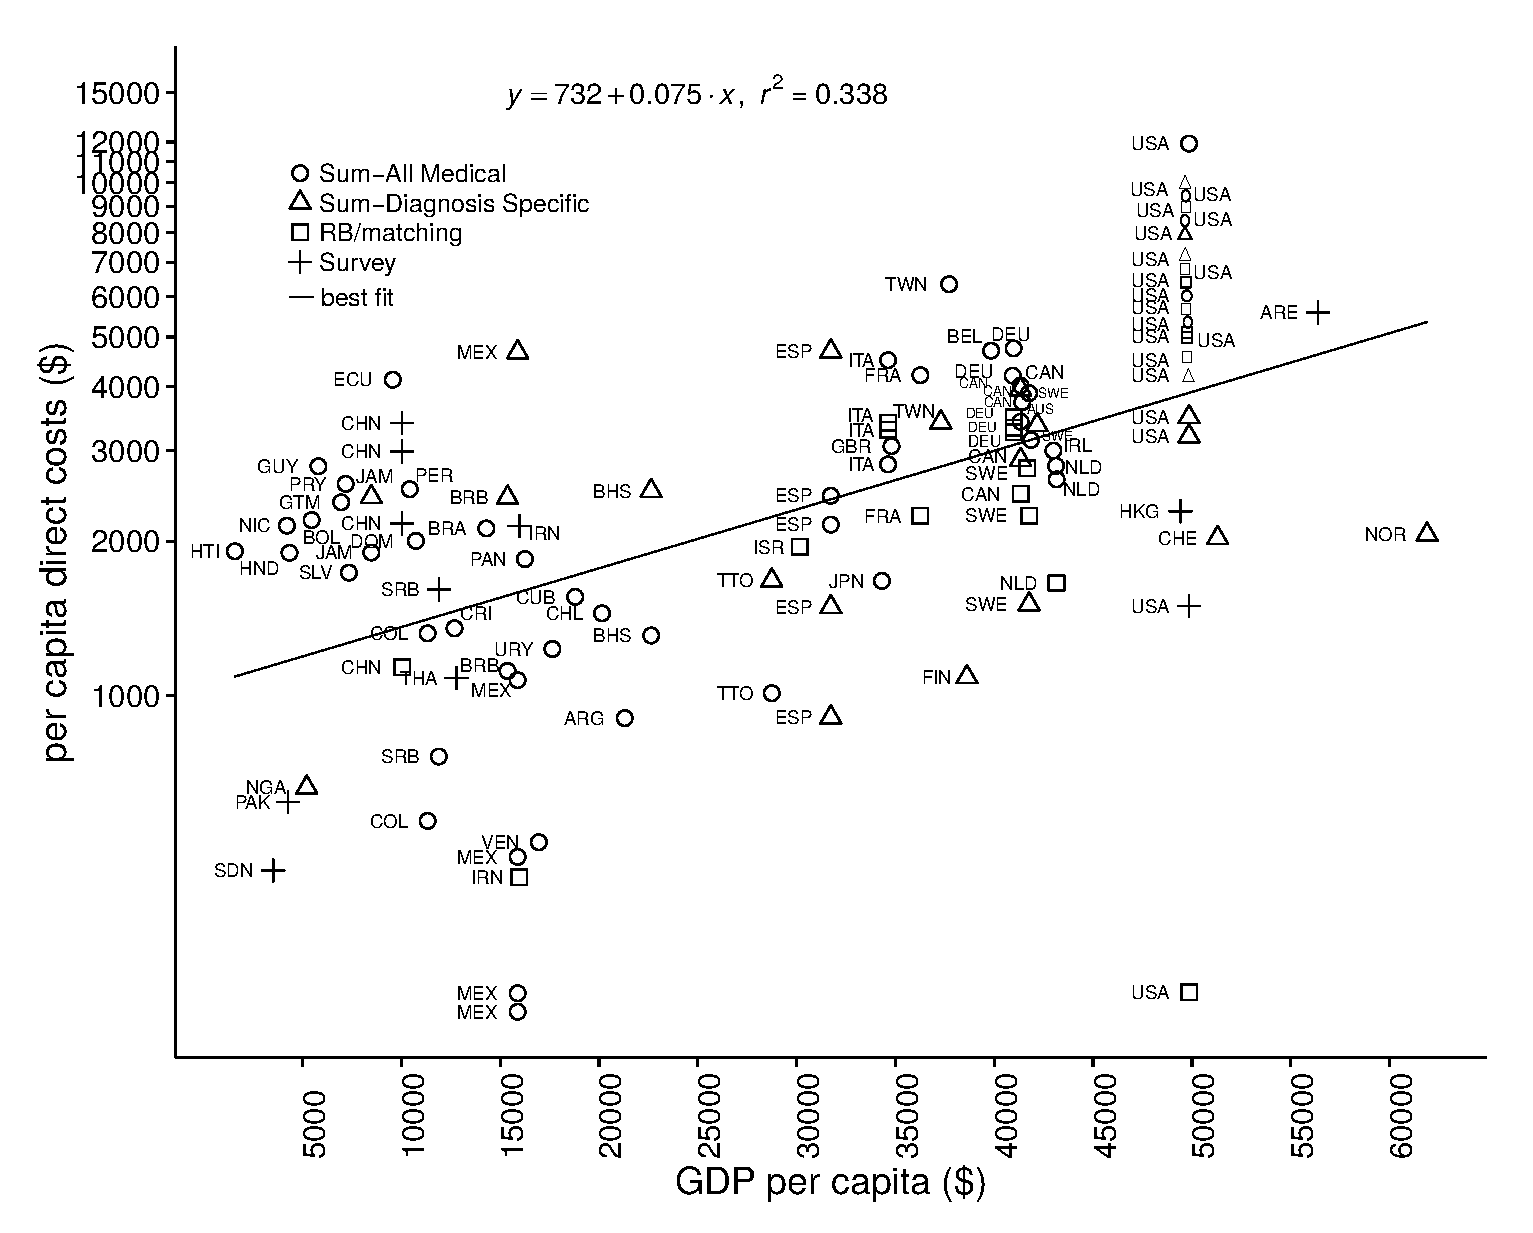
\includegraphics[width=1\linewidth]{Review/Figures/Fig3.eps}\\
\end{center}
\footnotesize
\textit{Notes}  The line depicts the best fit based on the linear regression of direct costs on \ac{GDP} per capita in international dollars.
\end{minipage}
\end{figure}




\begin{table}[h]
\caption{\label{tab:review_regression}Relationship between direct costs and study characteristics (robust linear regression).}
\begin{center}
\begin{adjustbox}{max width=\linewidth}
\begin{threeparttable}
{
\def\sym#1{\ifmmode^{#1}\else\(^{#1}\)\fi}
\begin{tabular}{l*{2}{SS}}
\toprule
                 &\multicolumn{1}{c}{Estimate} &\multicolumn{1}{c}{Std. Error} \\ \midrule
                Constant & 2133 & 1773.922 \\
                GDP per capita (\$) & .045\sym{**} & 0.017 \\
                Estimation Approach &  &  \\
                \hspace*{10mm}Sum-All medical (Ref.) & &  \\
                \hspace*{10mm}Sum-Diagnosis Specific & -413.880 &  528.766 \\
                \hspace*{10mm}RB/matching & -719.868 &  526.896 \\
                \hspace*{10mm}Survey & -689.806 & 671.020 \\
                At least four costing components & 702.966\sym{*} & 403.968 \\
                USA study & 3111.067\sym{***} & 533.534 \\
                Year of study &  &  \\
                \hspace*{10mm}\textless1995 (Ref.) &  &  \\
                \hspace*{10mm}1995-1999 & -1744.799 & 1632.498 \\
                \hspace*{10mm}2000-2004 & -816.647 & 1586.966 \\
                \hspace*{10mm}2005-2009 & -1021.685 & 1592.595 \\
                \hspace*{10mm}2010-2014 & -2744.739 & 1839.689 \\
                Study representative & -598.670 & 409.070 \\
                Complications & 666.803 & 414.727 \\
\midrule
                R-squared adj. & .559 &  \\
                N & 70 &  \\ 
 \bottomrule
\end{tabular}
\begin{tablenotes}
\item Standard errors in parenthesis. Ref. reference category.
\item \sym{*} \(p<0.10\), \sym{**} \(p<0.05\), \sym{***} \(p<0.01\).
\end{tablenotes}
}
\end{threeparttable}
\end{adjustbox}
\end{center}
\end{table}

The sensitivity of the cost results to the estimation approach was also examined by two studies that investigated the effect of different estimation techniques in diabetes \ac{COI} studies. \textcite{Honeycutt2009a} compared the use of a regression-based and an attributable-fraction approach and found that the cost estimate of the former exceeded the latter by 43 \%. \textcite{Tunceli2010c} compared the matching and the diabetes (disease)-attributable costs approach and found a 14--29 \% higher cost estimate using matching, depending on the used assumptions. Both studies concluded that an incremental cost approach results in a higher, and likely more exact, estimate of the direct costs of diabetes than disease-attributable approaches. The authors attributed this to the fact that a regression or matching approach can assign costs to diabetes that cannot be linked to diabetes otherwise. Those approaches are therefore in a position to account for all costs of co-morbidities caused by diabetes, while this is not automatically the case with the other approaches.

\subsubsection*{Direct and indirect costs of diabetes}

To assess the relative importance of direct and indirect costs across countries, we plotted direct against indirect costs from studies that provided both estimates and drew a 45\degree line depicting the equal share of direct and indirect costs (see Figure \ref{fig:review_direct_indirect}).

Most studies found a larger share for direct costs in comparison with indirect costs (observations above the 45\degree line in Figure \ref{fig:review_direct_indirect}). This is especially true for \acp{HIC}, where only a study on Sweden \parencite{Bolin2009d} found a larger share for indirect costs. For \acp{LMIC}, a study on Colombia \parencite{Gonzalez2009b} found considerably higher indirect costs, as did the multi-country study of \textcite{Barcelo2003} and a study on various countries in the African region \parencite{Kirigia2009}, which both found higher indirect costs for almost every country in the study and also on average for the entire regions, represented as the mean overall study estimate in Figure \ref{fig:review_direct_indirect}.  Both studies used similar approaches to estimate costs, and indirect cost estimates were likely so high because evidence from only a few countries within the region was used as a basis for estimating indirect costs for every other country in the respective study. Further, the studies took the countries' per capita gross national product as a proxy for earnings, which might have led to an over-estimation of the indirect costs \parencite{Kirigia2009}.

\begin{figure}[hp]
\caption{\label{fig:review_direct_indirect}Direct and indirect cost relation in studies estimating total costs of type 2 diabetes.}%
\begin{minipage}{\linewidth}
\begin{center}
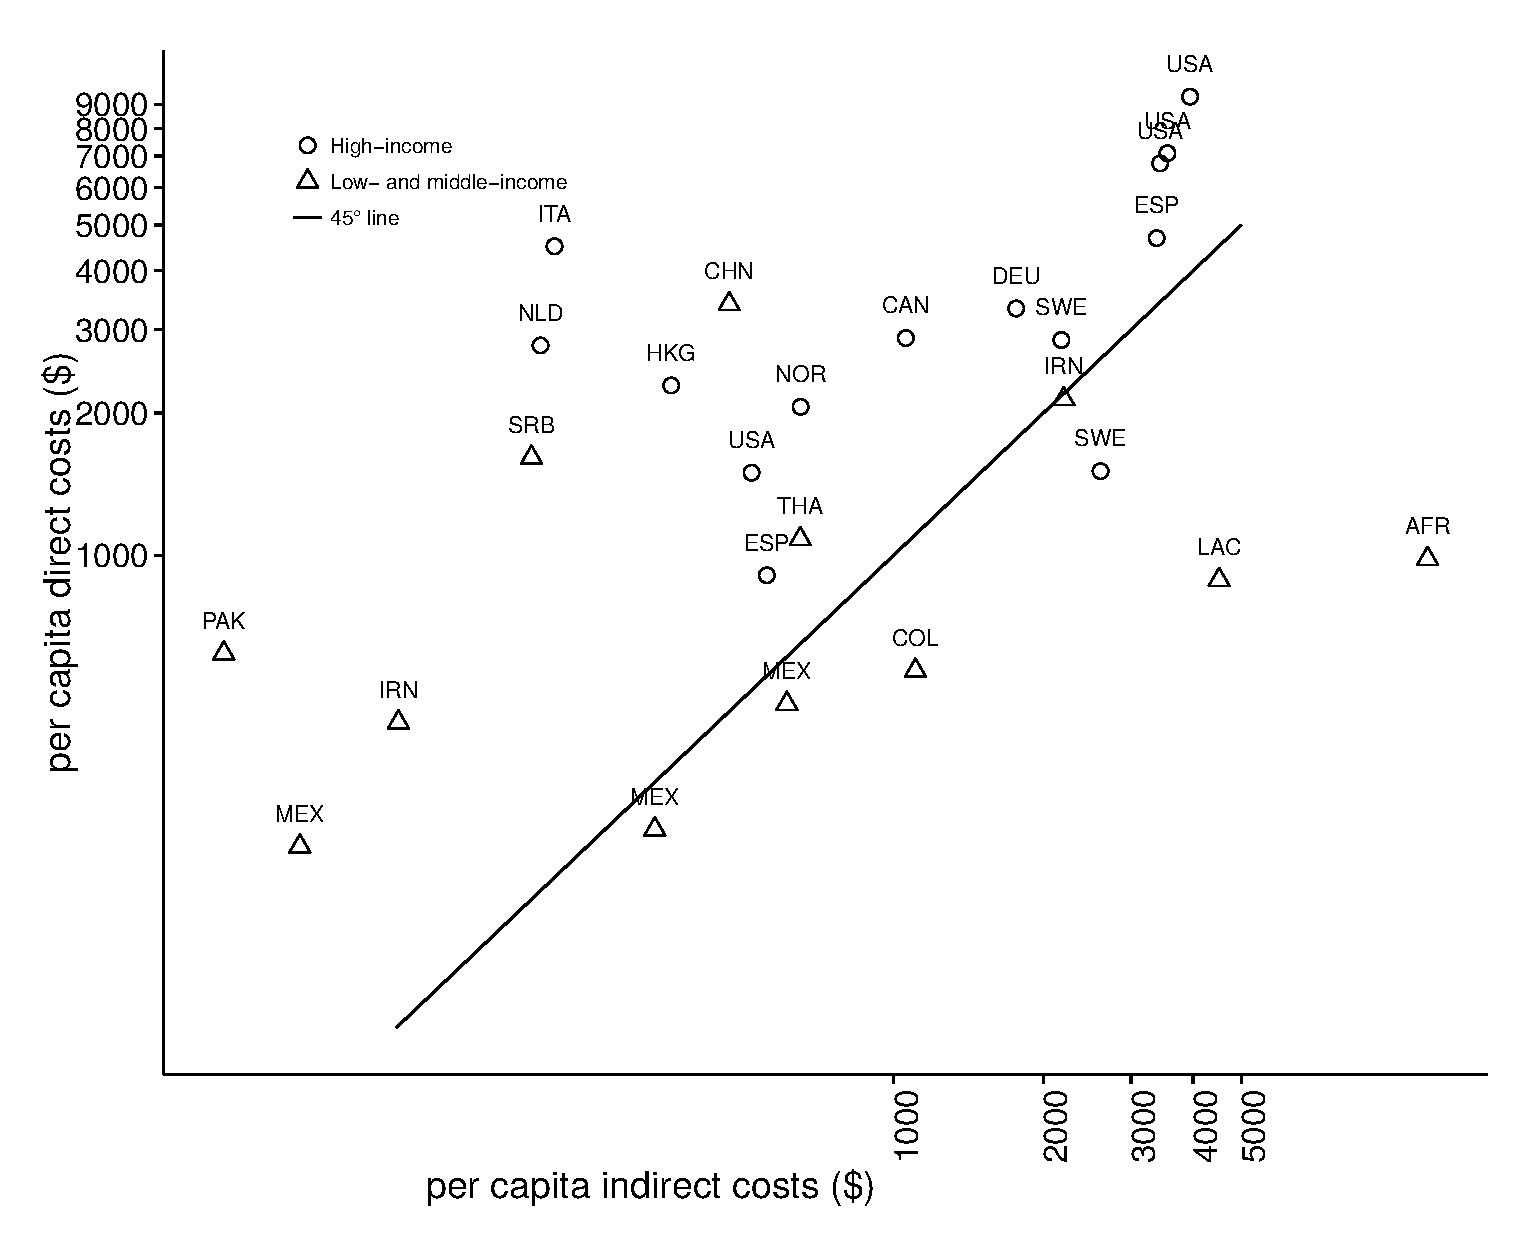
\includegraphics[width=1\linewidth]{Review/Figures/Fig4.eps}\\
\end{center}
\footnotesize
\textit{Notes} The 45\degree line depicts the points where direct and indirect costs would be equal. Above the line direct costs are higher than indirect costs and vice versa. For better visibility both coordinate axes are expressed in log scale
\end{minipage}
\end{figure}

\subsubsection*{Studies using the incidence approach}
The four studies that used an incidence approach (see Table \ref{tab:review_incidence} estimated the cost of diabetes either over a person's lifetime \parencite{Gonzalez2009b,Birnbaum2003c} or over a certain period after diagnosis \textcite{Johnson2006d,Martin2007b}. \textcite{Gonzalez2009b} modelled the lifetime (direct and indirect) costs of a typical diabetes patient in Colombia, arriving at a mean cost estimate of \$54,000. The second study providing lifetime estimates by \textcite{Birnbaum2003c}, estimated incremental lifetime healthcare costs for USA females with diabetes of \$283,000.


\begin{table}[hp]
\centering
\footnotesize
\begin{tabularx}{\linewidth}{X X X X X X}
\caption{Incidence studies on the costs of diabetes}\label{tab:review_incidence}\\
\toprule
Ref. &  Country & Time horizon & Population & Approach & Results \\ 
\midrule 
\textcite{Johnson2006d} &  Canada & 1992--2001 & Incidence T2D patients from Saskatchewan Health's administrative database in Canada & Sum-all medical & Highest  total healthcare costs at year of diagnosis with CAN\$7343 (\$7635), then increased from a low of CAN\$3880 (\$4034) 3 years after diagnosis to CAN\$4441   10 years thereafter (\$4618). \\
	\textcite{Gonzalez2009b} & Colombia & 32 years & Hypothetical average Columbian T2D patient & Sum-all medical & Total lifetime costs (32 year  period) of average diabetes patient, including direct and indirect costs,  57.565 million Colombian pesos (\$54,351). \\
\textcite{Martin2007b} & Germany & 1995--2003 & Newly  diagnosed T2D patients from randomly drawn practices across Germany & Sum-all medical & EUR 1,288   (\$1635) for the first treatment year after diabetes diagnosis and increased   to EUR 3845 (\$4880) in the seventh year. \\
\textcite{Birnbaum2003c} & United  States & 1997--1998 & Women employed by nationwide operating company and hypothetical women above age 64 receiving Medicare & RB/matching & \$282973 incremental lifetime direct healthcare costs, using incidence-based, steady-state methodology. \\ \bottomrule
\end{tabularx}
\end{table}



Two studies followed patients over a limited time period and found different patterns in the development of type 2 diabetes-attributable healthcare costs. In Germany costs increased from  \$1634 in the first year after diagnosis to \$4881 in the seventh year \parencite{Martin2007b}. In Canada, \textcite{Johnson2006d} found the highest costs in the year of diagnosis with \$7635, up from \$2755 the year prior to diagnosis. In the year after diagnosis costs decreased to \$4273 and then only increased slightly to \$4618 in year ten. In Germany and Canada, costs related to complications or hospital visits were the most important components and in Germany increased steadily over time. In Canada costs related to prescriptions increased the most.

\subsubsection*{Country level costs prediction studies}
Four studies projected costs of diabetes over a certain period of time \parencite{Ohinmaa2004,Lau2011a,Davis2006b,Wang2009f}, making assumptions about the future development of diabetes prevalence and population ageing (see Table \ref{tab:review_prediction}). For Canada, a 1.7-fold increase from 2000 to 2016 \parencite{Ohinmaa2004} and a 2.4-fold increase from 2008 to 2035 in diabetes healthcare costs was estimated \parencite{Lau2011a}. Taking a health care system perspective, both studies found that the estimated increase would be mostly driven by an ageing population. For Australia, \textcite{Davis2006b} estimated a 2.5- to 3.4-fold increase in diabetes attributable healthcare costs from 2000 to 2051, depending on the underlying assumptions about population ageing and diabetes prevalence rates. For China, \textcite{Wang2009f} extrapolated total costs of diabetes from the year 2007 to 2030, estimating the costs of diabetes to increase 1.8-fold, solely accounting for the expected increase in prevalence.

\begin{table}[hp]
\begin{tabularx}{\linewidth}{m m m m m b}
\caption{Country level costs prediction studies}\label{tab:review_prediction}\\
\toprule
Ref. & Country & Population   & Approach & Time  horizon & \multicolumn{1}{c}{Results}                                                                                                                                            \\ \midrule
\textcite{Davis2006b}  & Australia & Australian   population                       & Sum diagnosis  Specific & 2000--2051                                                              & If age and sex specific prevalence remains unchanged a 2.5-fold increase; if age and sex specific prevalence allowed to change as well a 3.4-fold increase. \\
\textcite{Ohinmaa2004}  & Canada    & Canadian   population                         & Sum-all   medical costs  & 2000--2016                                                              & 1.7-fold increase.                                                                                                                                          \\
\textcite{Lau2011a}  & Canada    & Four   Alberta Health and Wellness databases  & Sum-all  medical costs  & 2008--2035                                                              & 2.4-fold increase.                                                                                                                                          \\
\textcite{Wang2009f}  & China     & In   patients and outpatients in 20 hospitals & Own   survey             & 2007 and  2030 (projection) & Increase from \$73 billion in 2007 to \$132 billion in 2030 (1.8 fold increase).                                       \\ \bottomrule
\end{tabularx}
\end{table}

\subsection{The impact of diabetes on employment chances and productivity}
Besides studies that determined the cost of diabetes by costing related expenditures, another body of research has investigated---using econometric techniques---the impact of diabetes on 'productivity', a term used here to comprise outcomes including employment probabilities and lost work days and income or earnings. A recent study systematically reviewed evidence on the impact of diabetes on the ability to work, focusing on studies assessing the impact of diabetes on early retirement, lost work hours, absenteeism and presenteeism \parencite{Breton2013}. We focused particularly on studies exploring the impact of diabetes on employment probabilities and earnings---both issues that were not covered in the mentioned review---and we took a more detailed look at the empirical challenges posed by the issue of endogeneity (see the Appendix for a more detailed discussion of endogeneity).

Tables \ref{tab:rev_Diab_employment} and \ref{tab:rev_Diab_productivity} synthesize the relevant information from the 23 identified studies on the effect of diabetes on employment and other labour market outcomes. Almost all studies were conducted on \acp{HIC}, mainly the USA (n=13) and European countries (n=4). Only one study focused on a \ac{LMIC}. investigating the effect of diabetes on labour income in China.

\subsubsection*{Employment chances}
Most studies examined the impact of diabetes on employment probability (n=17), applying a range of econometric techniques. These have evolved over time, and more recent studies took into account the possibility that diabetes might be endogenous: it is conceivable that especially personal traits such as motivation and drive could influence the propensity to develop type 2 diabetes as well as a persons' job market opportunities. Further, being employed or unemployed could also lead to changes in lifestyles, due to changes in income, stress or leisure time, that could themselves affect the chances of developing diabetes \parencite{Brown2005}. Of the studies that tried to account for this problem \parencite{Brown2005,Minor2011,Latif2009,Lin2011b,Zhang2009,Harris2009}, the majority used an \ac{IV} technique. This approach allows for the consistent estimation of the effect of diabetes on employment if a variable can be found that is causally related to diabetes without affecting the employment chances through any other unobserved pathway apart from its effect on diabetes (see Text Box 1). In the case of type 2 diabetes all studies used the family history of diabetes as an \ac{IV} to exploit the fact that the development of type 2 diabetes is much more likely for individuals whose biological parents have also had diabetes. It is argued that, while controlling for education, age and other observable demographic and socioeconomic factors (e.g. wealth, regional and ethnic differences and the number of children in the household), having a family member with diabetes should not affect the person's employment status or other labour market outcomes, while strongly predicting the onset of type 2 diabetes. 


\begin{tabularx}{\linewidth}{m m m m b b}
\caption{Studies estimating the relationship between diabetes and employment (2001 -- 2014)}\label{tab:rev_Diab_employment}\\
\toprule
Ref & Survey year & Country  & Age     & \multicolumn{2}{c}{Effect on employment} \\ \cmidrule(l){5-6}                                                                                                                                                                                                                                                                                                                                                                              &  &  &   & \multicolumn{1}{c}{Males} & \multicolumn{1}{c}{Females} \\ \midrule \endfirsthead
\caption[]{Studies estimating the relationship between diabetes and employment (2001 -- 2014)}\\
\toprule
Ref & Survey year & Country  & Age     & \multicolumn{2}{c}{Effect on employment} \\ \cmidrule(l){5-6}                                                                                                                                                                                                                                                                                                                                                                              &  &  &   & \multicolumn{1}{c}{Males} & \multicolumn{1}{c}{Females} \\ \midrule \endhead
\textcite{Harris2009} & 1999-2000      & Australia                                                                                 & \textgreater24              & Exogenous: 10.8 percentage points reduction to be in labour force; endogenous: 7.1 percentage points reduction and test indicates endogeneneity.                                                                                                           & Exogenous: 10 percentage points to be in labour force; endogenous: Nine percentage points reduction and test indicates endogeneneity.                                    \\
\textcite{Zhang2009} & 2001, 2004-2005 & Australia                                                                                 & 18-64                       & 50-64: 11.5 percentage points less likely to be in labour force; 18-49: 3.9 percentage points less likely, all effects increase when other chronic diseases are present.                                                                                   & No significant effect for diabetes alone; significant negative effect if other chronic diseases are present.                                                             \\
\textcite{Latif2009} & 1998           & Canada                                                                                    & 15-64                       & Exogenous: 19 percentage points less likely to be employed; endogenous: not significant and positive and test indicates endogeneity.                                                                                                                       & Exogenous: 17 percentage points less likely to be employed, endogenous: not significant and positive and test indicates exogeneity.                                      \\
\textcite{Kraut2001a} & 1983-1990      & Canada                                                                                    & 18-64                       &\merge{With complications 2 times less likely to be in labour force; no significant effect on employment for those in labour force.\textsuperscript{a}} \\
\textcite{Norlund2001a}  & 1992-1993      & Sweden                                                                                    & \textgreater24              & \merge{14.2 percentage points higher retirement rate (22.9 compared to 8.7).\textsuperscript{a}} \\
\textcite{Alavinia2008a} & 2004           & Sweden, Denmark, Netherlands, Germany, Austria, Switzerland, France, Italy, Spain, Greece & 50-65                       & \merge{For whole dataset: no effect of diabetes on being unemployed, but increased odds ratio of 1.33 on being retired. No information on effects by country.\textsuperscript{a}} \\
\textcite{Lin2011b} & 2005           & Taiwan                                                                                    & 45-64                       & Exogenous: 9 percentage points less likely to be employed; endogenous: 19 percentage points less likely to be employed; test on whole sample indicates endogeneity.                                                                                        & Exogenous: 11 percentage points less likely to be employed, endogenous: not significant and negative.                                                                    \\
\textcite{Brown2005}  &                & United States                                                                             & \textgreater44              & Exogenous: 7.4 percentage points less likely to be employed; endogenous: 10.6 percentage points less likely but test indicates exogeneity.                                                                                                                 & Exogenous: 7.5 percentage points less likely to be employed; Endogenous: no significant effect found and test indicates endogeneity.                                     \\
\textcite{Minor2011}  & 2006           & United States                                                                             & \textgreater19 at diagnosis &                                                                                                                                                                                                                                                            & Exogenous: 25.2 percentage points less likely to be employed, endogenous: 45.1 percentage points less likely to be employed.                                             \\
\textcite{Vijan2004} & 1992-2000      & United States                                                                             & 51-61                       & \merge{More likely to be retired in 1992 (adjusted OR 1.3). Over 8 years follow up spent 0.14 incremental years in retirement.\textsuperscript{a}}\\
\textcite{Bastida2002} & 1996-1997      & United States                                                                             & \textgreater44              & 7.5 percentage points less likely to be employed.                                                                                                                                                                                                          & No significant effect on employment chances found.                                                                                                                       \\
\textcite{BrownIII2011} & 2008           & United States                                                                             & 35-64                       & Diabetes negatively related to employment (5 percentage points reduction); better diabetes management (\ac{HbA1c}) positively affects employment probabilities; \ac{HbA1c} lowering of 10\% increases employment probability by 0.44 percentage points.                  & No significant effect on employment chances found.                                                                                                                       \\
\textcite{Tunceli2005a} & 1992,1994      & United States                                                                             & 51-61                       & 9 percentage points less likely to work without complications controlled for, with complications controlled for 7.1 percentage points less likely.                                                                                                         & 5.9 percentage points less likely to work without complications controlled for, with complications controlled for 4.4 percentage points less likely but not significant. \\
\textcite{Tunceli2009a} & 1997-2005      & United States                                                                             & 20-44 and 45-64             & \merge{20-44: proportion with work limitations 3.1\% higher; 45-64: proportion not working is 8.1\% higher; the proportion work disabled is 3.4\% higher; proportion with work limitations is 5.7\% higher (all compared to similar age group without diabetes).\textsuperscript{a}}\\
\textcite{Valdmanis2001} & 1990-1995      & United States                                                                             &                             & \merge{Unemployment rate for persons with diabetes was 16\% compared with 3\% among matched comparison group.\textsuperscript{a}} \\
\textcite{Ng2001b} & 1989           & United States                                                                             & \textgreater29 at diagnosis & \merge{3.6\% less likely of being employed (exogenous), 12\% for those with complications.\textsuperscript{a}}                                                                                                                                                                                                                                                                                                                                              \\
\textcite{Minor2013} & 1979-2010      & United States                                                                             & \textgreater14              & Average reduction of employment probability of 28 percentage points; strongest employment penalty in first 5 years after diagnosis.                                                                                                                        & Average reduction of employment probability of 36 percentage points; strongest employment penalty in first 15 years after diagnosis.                                     \\ \bottomrule
\multicolumn{6}{l}{\footnotesize \textsuperscript{a} No gender differentiation in study}
\end{tabularx}



Because \ac{IV} estimation has worse asymptotic properties than single equation regression results when endogeneity is not an issue, studies tested for the existence of endogeneity to determine which results to rely on for inference \parencite{Brown2005,Minor2011,Latif2009,Lin2011b}. Interestingly, the reviewed studies found diabetes to be endogenous for either males \parencite{Latif2009} or females \parencite{Brown2005,Minor2011}, but never for both. Further, the use of an \ac{IV} sometimes increased the estimated effect\parencite{Minor2011,Lin2011b} whereas in other cases the effect turned insignificant \parencite{Brown2005,Latif2009}. As a result, no unambiguous conclusions can be drawn as to how endogeneity affects diabetes and whether or not it causes biased estimates. Most of the relevant studies also explored whether accounting for \ac{BMI} or other diabetes-related chronic conditions would substantially alter the result and found this not to be the case \parencite{Brown2005,Latif2009,Minor2013}.

Overall, studies more commonly found a significant adverse impact of diabetes on males, ranging from no effect in Canada \parencite{Latif2009} to a 19 percentage point reduction in Taiwan \parencite{Lin2011b}. Conversely, no effect was found for women in Taiwan  \parencite{Lin2011b}, Australia  \parencite{Zhang2009} or for Mexican Americans in Texas \parencite{Brown2005}. However, a 45 \% decrease in employment chances was observed for women in the USA \parencite{Minor2011}. Extending the scope and looking at how diabetes duration affected labour market outcomes, using pooled longitudinal data from the USA, one study found that the main adverse effect on employment chances materialized within the first 5 years after diagnosis for men and 11--15 years after diagnosis for women \parencite{Minor2013}.

\subsubsection*{Productivity}
For earnings, no effect was found for Mexican-American men in Texas \parencite{Bastida2002}, while the highest loss was found for women in the USA (\$21392 per year) \parencite{Minor2011}. Again looking at diabetes duration, a wage penalty was only found for USA men 6--10 years after diagnosis, reducing their wage by about 18 percentage points \parencite{Minor2013}. The only study on a non-\ac{HIC}, China, tried to tease out the psychological effect of a diabetes diagnosis on subsequent labour income, finding a reduction of 22 \% in income for males, but not for females. Further, those with an \ac{HbA1c} between 8--10 \% experienced the most severe income penalty (29 \%). The study further showed that the adverse effect of a diabetes diagnosis was concentrated among the poorest third of the study population \parencite{Liu2014}. Another study investigated the effect on earning losses for caregivers of people with diabetes in the \ac{UK}, finding a reduction of \$2,609 per year, while the person with diabetes experienced a loss of \$1,744 per year \parencite{Holmes2003a}. For income, a reduction of \$6,250 per year was found for older USA adults who had been followed between the years 1992 and 2000 \parencite{Rivera2004}. In terms of lost workdays and work hours due to diabetes, the effects ranged from no impact on lost work days on older people \parencite{Rivera2004} and females in the USA \parencite{Minor2011} to 3.2 lost work days in a USA population within a 2-week period if complications were present \parencite{Ng2001b}.



\begin{tabularx}{\linewidth}{m m m m  b b}
\caption{Studies estimating the relationship between diabetes and other productivity outcomes (2001 -- 2014)}\label{tab:rev_Diab_productivity}\\
\toprule
Ref.      & Survey year & Country        & Age                               & \multicolumn{2}{c}{Effect on other productivity outcomes} \\ \cmidrule(l){5-6}
          &             &                &                                   & \multicolumn{1}{c}{Males}                                                                                                                                                                                                                                 & \multicolumn{1}{c}{Females}                                                                                                                                                                                                                             \\ \midrule \endfirsthead
 \caption[]{Studies estimating the relationship between diabetes and other productivity outcomes (2001 -- 2014)}\\
          \toprule
          Ref.      & Survey year & Country        & Age                               & \multicolumn{2}{c}{Effect on other productivity outcomes} \\ \cmidrule(l){5-6}
                    &             &                &                                   & \multicolumn{1}{c}{Males}                                                                                                                                                                                                                                 & \multicolumn{1}{c}{Females}                                                                                                                                                                                                                             \\ \midrule \endhead
\textcite{Kraut2001a} & 1983--1990 & Canada & 18--64 & Effect on earnings only when complications are present: reduced to 72\% of total income of controls.a &  \\
\textcite{Liu2014} & 2009, 2011 & China & not given &  \merge{16.3\% decrease in annual income; strongest effect for those in lower income quintiles.\textsuperscript{a}} \\
\textcite{Herquelot2011} & 1989--2007 & France & Male 40--50, females 35--50 in 1989 & \merge{1.7 HR to transition from employed to disabled, 1.6 HR to be retired, 7.3 HR to be dead; between age 35 and 60 each person with diabetes lost 1.1 years of time in workforce.\textsuperscript{a}} \\
\textcite{Leijten2014a} & 2010--2013 & Netherlands & 45--64 & \merge{Diabetes reduced work ability measured using Work Ability Index (WAI) by 2\%. No significant effect on productivity was found.\textsuperscript{a}} \\
\textcite{Norlund2001a} & 1992--1993 & Sweden & \textgreater24 & \merge{9.4 more sick days.\textsuperscript{a}} \\
\textcite{Holmes2003a} & 1999 & United Kingdom & \textless65 & \merge{GBP 869 lost earnings per year with diabetes; GBP 1300 for carers of people with diabetes.\textsuperscript{a}}\\
\textcite{Minor2011} & 2006 & United States & \textgreater19 at diagnosis &  & Exogenous: \$2865 loss in earnings per year, Endogenous: \$19655; Exogenous: 2 working hours less per week, no significant effect on missed workdays per year, endogenous: no significant effect on working hours or workdays missed. \\
\textcite{Vijan2004} & 1992--2000 & United States & 51--61 & \merge{Lost income of \$50004 from 1992--2000 per capita or \$6250 per year, for whole USA population of same age  \$85.6 billion or \$10.7 billion per year; people with diabetes more likely to have taken sick days in 1992 (adjusted OR 1.3).\textsuperscript{a}} \\
\textcite{Collins2005} & 2002 & United States & working age & \merge{No significant effect on work days.\textsuperscript{a}} \\
\textcite{Bastida2002} & 1996--1997 & United States & \textgreater44 & No significant effect on earnings. & Women with diabetes earn 84\% less. \\
\textcite{BrownIII2011} & 2008 & United States & 35--64 & Wages reduced by 0.74\% due to diabetes; for every 10\% reduction in A1C wages rise by 0.62 \%. A1C \textgreater 8 was related to decreasing wages. & No significant effect of diabetes on female earnings; no effect of blood sugar management for women, A1C levels just below 6 to just above 7 were related to lower wages. \\
\textcite{Lenneman2011} & 2005--2009 & United States & \textgreater16 & \merge{Lost earnings per year of \$2146.\textsuperscript{a}}  \\
\textcite{Tunceli2005a} & 1992, 1994 & United States & 51--61 & No significant effect on number of work days. & 2.5 more lost workdays per year. \\
\textcite{Valdmanis2001} & 1990--1995 & United States &  & \merge{71\% of the persons with diabetes had an annual income of less than \$20000 compared with 59\% of the matched respondents.\textsuperscript{a}} \\
 &  &  &  &  &  \\
\textcite{Ng2001b} & 1989 & United States & \textgreater29 at diagnosis & No significant effect on work days for T2D, for those with complications 3.2 days lost within two weeks &  \\
\textcite{Brown3rd2005b} & NA & United States & \textgreater45 & \merge{For every dollar of labor income lost by adults with diabetes, a further income reduction of \$0.48  occurs in the community. Total output reduction for upper bound estimate is \$300 million for the local economy.\textsuperscript{a}} \\
\textcite{Minor2013} & 1979--2010 & United States & \textgreater14 & no general effect of type 2 diabetes on wages; some evidence of wage penalty of about 18\% 6--10 years after diagnosis & No strong evidence found for wage penalty for females \\ \bottomrule
\multicolumn{6}{l}{\footnotesize \textsuperscript{a} No gender differentiation in study}
\end{tabularx}

In terms of the methodology used, these studies tended to rarely account for endogeneity, and they mostly used standard regression or matching methods to estimate the impact of diabetes. Three studies \parencite{Minor2011,Bastida2002,BrownIII2011} corrected for the possibility of a sample selection bias, to account for systematic differences between the working population and the overall population. Only one study additionally applied \ac{IV} methods and found diabetes to be endogenous, so that its effects on earnings were dramatically understated using naive regression results \parencite{Minor2011}. For working hours and days missed due to illness, the same study found no indication of endogeneity. Only one study applied an approach other than \ac{IV} to account for endogeneity, using a difference-in-difference model and exploiting a recent diagnosis of diabetes, which was the result of the collection of biomarkers in the survey used, as a natural experiment to measure how income developed between those who were newly diagnosed and those without diabetes in the years following diagnosis \parencite{Liu2014}.

\section{Discussion}
The objectives of this systematic review were to identify new evidence on the economic impact of type 2 diabetes that emerged since 2001 and extend the scope of the review by including studies on the labour market impact of diabetes. We identified studies from a great variety of countries, with large differences in cost estimates across and within countries.

\subsection{General findings and developments since the 2004 review of diabetes COI studies}
An obvious development since the last review is the emergence of \ac{COI} studies on \acp{LMIC}. The economic burden related to diabetes found in these studies indicated a strong direct impact on those affected by diabetes. This is reflected in the substantial burden of \ac{OOP} treatment costs incurred by patients \parencite{Smith-Spangler2012,Suleiman2006,Arredondo2007,Esteghamati2009,Wang2009b,Ramachandran2007d,Khowaja2007a,Elrayah-Eliadarous2010b,Chatterjee2011c,Tharkar2010a,Wang2010c}, with considerable proportions of the annual income being spent on diabetes care. This relative cost burden was generally higher for people with relatively lower household incomes \parencite{Ramachandran2007d,Khowaja2007a,Tharkar2010a}. Health insurance coverage had some protective effects against \ac{OOP} expenditures, but mainly for those with higher incomes, while the poor often lacked coverage \parencite{Ramachandran2007d,Khowaja2007a,Tharkar2010a}.Nonetheless, once people were covered by health insurance their risk of incurring catastrophic expenditures decreased significantly \parencite{Smith-Spangler2012}. An important cost factor that was predominantly investigated in studies on \acp{LMIC} were non-medical costs for transportation, informal healthcare or food which were found to considerably add to the experienced diabetes cost burden \parencite{Esteghamati2009,Wang2009b,Wang2009f,Chatterjee2011c,Tharkar2010a}.

In terms of the costing methodology applied in \ac{COI} studies, the number of studies estimating the excess costs of diabetes increased since the \textcite{Ettaro2004} review. Those studies either used regression analysis or matching to adjust for the differences between people with diabetes and those without, accounting at least for age and gender, but often also for other socioeconomic, geographic and demographic differences. Other widely used approaches to estimate direct healthcare costs from the perspective of the healthcare system or private insurance included the disease-attributable and---slightly less frequently---the attributable-fraction approach. For cost assessment in \acp{LMIC}, studies often either estimated total healthcare costs or carried out self-administered surveys. While \textcite{Ettaro2004} recommended the use of disease-attributable approaches to arrive at more exact estimates of the costs of diabetes, the evidence found in this review indicates that using an incremental cost approach via matching or regression analysis could provide more accurate results, due to its ability to capture costs otherwise not directly traceable to diabetes. Nonetheless, the use of the estimation technique always hinges on the availability of appropriate data, with regression or matching analyses requiring information on people without diabetes to be used as a control group. Therefore the estimation approach needs to be tailored to the available data. 

Compared with the evidence reviewed by \textcite{Ettaro2004}, the field has generally advanced with respect to the analysis of costs in different ethnic and age groups. Two studies investigated differences between racial groups in the USA, showing that while ethnic minorities spend less on diabetes healthcare than Whites, this difference seems to be mainly based on differences in access to care between Whites and Blacks or Hispanics \parencite{Lee2006,Buescher2010}. In terms of age, studies found an increase in healthcare costs with age as well as with, in some cases, the duration of diabetes. A recurring problem was that many studies did not distinguish diabetes types, making it difficult to exactly attribute the costs to the respective diabetes types.

To explore the reasons for the wide heterogeneity in direct cost estimates across studies, we performed a regression analysis, which indicated that an important determinant for the cost variation across countries could be the economic wealth of the country (proxied by \ac{GDP} per capita), similar to what was found in a review of indirect costs of various chronic diseases \parencite{Zhao2013}, possibly due to differences in the availability and affordability of diabetes care between \acp{HIC} and \acp{LMIC}  \parencite{Cameron2009g,Cameron2011b}. 

Further, studies on the USA seem to estimate consistently higher costs than studies on other countries, even when accounting for differences in \ac{GDP} per capita. The higher direct costs of diabetes estimated for the USA are in line with the generally higher healthcare expenditures in the USA compared with countries with similar income levels, and could be the result of exceptionally high service fees \parencite{Laugesen2011} and prices paid in the USA healthcare system \parencite{Squires2012,Lorenzoni2014}.

Because of the small sample size on which our analysis was based, these results must be interpreted with caution, and other factors could still be important. For instance, other evidence suggests that different costing approaches have a considerable effect on diabetes cost estimates \parencite{Tunceli2010c,Honeycutt2009a}. Furthermore, the perspective taken, different data sources and populations investigated and decisions on the cost components included are likely important in explaining within-country heterogeneity. In particular, the inclusion of diabetes complications and decisions about which complication(s) to include, as well as the extend to which costs for these diseases are attributable to diabetes, can significantly affect the results. Not all studies in the review provide extensive information about how they include complications and some do not include them at all.

Finally, the quality of the data used could have affected the cost estimates. Many studies in \acp{LMIC} relied on self-reported data from small household surveys, limiting their generalizability and leading their results to be prone to recall bias. Further, these studies often identified people with diabetes via their use of healthcare institutions, which excluded a potentially important section of the population in \acp{LMIC} unable to access formal care, possibly leading to an overestimation of the average diabetes-related costs. 

\subsection{Labour market studies}
Turning to the effects of diabetes on the labour market, the existing studies showed, almost consistently, with the exception of Canada \parencite{Latif2009} and one study on the USA \parencite{Minor2013}, that the employment probabilities of men were affected more adversely by the disease than those of women. However, while most studies have tried to tentatively explain these gender differences, the reasons for this have not been investigated in depth.  The studies also showed that, when interpreting this research, it is important to consider whether a study has tried to account for unobservable factors or reverse causality, as otherwise the results might be misleading. Nonetheless, all studies using \ac{IV} techniques used similar instruments to achieve identification, providing scope for further research using different identification strategies to explore how endogeneity might affect the results. What has been apparent is the lack of research on labour market outcomes of diabetes in \acp{LMIC}, with only one study investigating the effect of diabetes on labour income in China \parencite{Liu2014}. This deficit might be due to a limited availability of suitable data sources containing sufficient information to allow for a similar investigation of the topic.

The potential for rich, good-quality data sources to aid the investigation of the economic impact of diabetes can be illustrated by the several studies that used data from the Lower Rio Grande Valley in Texas. These studies demonstrate the evolution of methodology and data from the use of single equation regression models \parencite{Bastida2002} to the use of \ac{IV} methods \parencite{Brown2005} and---finally---biometric data on blood glucose values \parencite{BrownIII2011}. While the first two methods allowed the investigation of the general effect of diabetes on employment chances, the latter was able to assess the impact according to how diabetes was managed by the patient, as proxied by the measured biomarkers. The study found that the main adverse effect was due to having diabetes regardless of how it was managed and that improvements in management only had minor positive effects. The authors concluded that investments in the prevention of diabetes would likely be more effective than improved diabetes management.

The latter study and the study by \textcite{Liu2014} also show how biometric data (e.g. blood glucose values) can be used to arrive at a deeper understanding of the economic effects of diabetes. Biometric information makes it possible to investigate the impact of diabetes according to the severity of the disease and also allows for the consideration of previously undiagnosed people with diabetes, increasing the policy relevance of the research.

\subsection{Comparison of COI and labour market studies: common themes and lessons learned}
The results of both fields, \ac{COI} and labour market studies, show a considerable adverse impact of diabetes in terms of costs to society, health systems, individuals and employers and in terms of a reduction in the productive workforce and productivity in general. Both research strands particularly indicate that the adverse effects of diabetes increase with diabetes duration as well as with the severity of the disease, judged by the high complication costs estimated in \ac{COI} studies and the larger employment and income penalties for those with a longer disease duration or higher blood glucose levels. 

Nonetheless, several lessons can be learned for each field from advancements in the other field. Future \ac{COI} studies would, for instance, benefit from the more frequent use of biomarker data. This would allow for a more precise analysis of the costs of diabetes according to the severity of the disease and help inform researchers and policy makers about the possible economic effects of achieving certain treatment goals, e.g., a reduction in blood glucose values.

Also, and in contrast to the labour market outcomes literature, the endogeneity problem has hitherto not been addressed in any form in studies estimating direct healthcare or productivity costs, despite it being an equally important challenge in this domain. A possible bias could arise if some people developed diabetes as a result of an unobserved accident or illness, likely resulting in an overestimation of the costs. Endogeneity could also be introduced if people with diabetes became poorer as a result of the disease and consequently were not able to spend as much on their treatment as they would like to, leading to an underestimation of the true monetary cost of diabetes. Furthermore, an endogeneity bias would be introduced if diabetes was correlated with poverty so that diabetes prevalence would be disproportionately high in subgroups with less resources and consequently less access to care. This would lead to an underestimation of the healthcare costs of diabetes. Endogeneity in \ac{COI} studies has recently been addressed for the estimation of healthcare costs of obesity, suggesting that direct costs would have been underestimated, had the study not accounted for endogeneity \parencite{Cawley2012b}. It appears that, on the basis of the studies identified in our review, a similar---worthwhile---approach could and should be applied to the case of type 2 diabetes.

Yet the labour market studies also stand to gain from adopting certain approaches that are more common in \ac{COI} studies. To date, only few labour market studies have used the incidence approach found for \ac{COI} studies to follow people with diabetes over a certain time period from their diagnosis onwards, in order to further explore how the effect of diabetes on employment and productivity measures develops over time.

Some further recommendations may be derived for future \ac{COI} and labour market studies on diabetes: 
\begin{enumerate}


\item	For \ac{COI} studies the estimation of incremental costs---wherever possible---appears to be most suitable for diabetes, as it more accurately accounts for costs of co-morbidities  and for less obviously related disease costs \parencite{Honeycutt2009a,Tunceli2010c}. More information that can guide researchers in their choice of methods already exists and should be referred to when performing a \ac{COI} study \parencite{Akobundu2006}.

\item	If possible, the use of convenience samples of people with diabetes visiting a health care institution should be avoided, particularly in \acp{LMIC}, as it excludes those not able or willing to visit a clinic for treatment due to economic reasons, leaving out a potentially important proportion of diabetes patients.

\item	The interpretation of the \ac{COI} results always hinges on the amount of information provided about, among others, the aim of the study, the perspective adopted and the cost components included as well as the estimation approach used. A discussion of how these choices might affect the estimates should also be part of every \ac{COI} study. Researchers should therefore consult available guidance from the literature that sets out what information should ideally be included in a \ac{COI} study \parencite{Larg2011} to increase the transparency and usability of their research. 

\item	For labour market studies more evidence from \acp{LMIC} is needed. There is scope for for exploring existing household datasets from \acp{LMIC} that contain information on diabetes \parencite{Seuring2014}. In some cases, panel data are (or may come) available, which would allow the investigation of the effects of diabetes over time as well as to improve the degree of causal inference by controlling for unobserved heterogeneity.

\item	As for labour market studies, other ways of achieving identification should be explored to reduce the reliance on \ac{IV} methods using the family history of diabetes as the sole instrument. The increasing richness of information provided in recent data sets could be used to this effect, also taking into account other quasi-experimental econometric methods \parencite{Craig2012}.
\end{enumerate}

\subsection{Limitations}
A possible limitation of this review is the decision to refrain from excluding studies based on certain quality criteria, such as study design, costing methodology, sample size or reporting standards. This might have resulted in the inclusion of lower quality studies with less reliable estimates, compromising the comparability across countries, particularly between \acp{LMIC} and \acp{HIC}, as study designs differed considerably. On the other hand our overarching objective was to ensure a truly globally comprehensive overview of the literature on the economic impact of diabetes, including evidence from \acp{LMIC}, which, for reasons often beyond the control of the researchers, may have been of limited quality and thus would have been excluded, had we applied stringent quality benchmarks. Further, any attempt to apply a quality threshold would have faced the challenge of dealing with the absence of a formal checklist to follow in critically appraising the quality of \ac{COI} studies. Rather than interpreting it as a limitation, we see the identification and synthesis of \ac{LMIC} studies as a unique added value of this review, when compared to the \textcite{Ettaro2004} review. 

Notably, we also abstained from any language restrictions, which would have particularly excluded evidence from Spanish speaking and Eastern European countries. Taken together, these factors have resulted in a large number of included studies, allowing for an (albeit exploratory) statistical investigation of the heterogeneity in diabetes cost estimates as a complement to the narrative analysis. We therefore feel that the advantages of refraining from too stringent inclusion criteria more than outweigh the possible negative consequences of including potentially lower-quality studies.

Further, our search was limited to studies after the year 2000. While for \ac{COI} studies a previous review covered the literature until 2000, this is not the case for the literature on labour market effects of diabetes and we therefore cannot exclude the possibility of having missed some relevant (if old) studies. We have checked the references of our included labour market
studies for any relevant studies published before 2001. We could find only one relevant study from 1998 investigating how employment
chances and family income were affected by diabetes in the USA, comparing samples from 1976, 1988 and 1992 and finding significant
adverse effects of diabetes on employment chances but not on family income \parencite{Kahn1998b}. The effect for women decreased somewhat between 1976 and 1992, while the effect increased for men. The study did not account for the possible endogeneity of diabetes nor selection bias when estimating the effects on income.

\section{Conclusion}

This review has provided an updated and considerably expanded picture of the literature on the global economic impact of type 2 diabetes. The results show a considerable impact of diabetes in terms of costs to society, health systems, individuals and employers and in terms of a reduction in the productive workforce and productivity in general. Studies on the costs of diabetes now provide evidence from \acp{HIC} as well as \acp{LMIC}, using a variety of study designs to estimate the costs of diabetes. The evidence indicates a particularly strong and direct economic impact of type 2 diabetes on people's livelihoods in lower-income settings. Studies on labour market outcomes so far have been confined, almost exclusively, to \acp{HIC}, leaving space for further studies in \acp{LMIC} to provide additional evidence of the effect of diabetes in these countries. An issue not yet covered in diabetes \ac{COI} studies---in striking contrast to labour market outcome studies---has been the possible bias introduced by endogeneity, providing an opportunity for advancing research in this area. 
\clearpage
\section*{What is endogeneity?}
Endogeneity is a statistical problem that occurs in regression models if the assumptions about the flow or direction of causality are incorrect. If endogeneity is ignored, it could be that claims about causality between two variables or the magnitude of the effect are false. In general, one can only be certain about a causal relationship of the effect of x on y if the following three conditions are met \parencite{Antonakis2012}:

\begin{itemize}
\item	y follows x temporally
\item	y changes as x changes (and this relationship is statistically significant)
\item	no other causes should eliminate the relation between x and y.
\end{itemize}

There are three major causes of endogeneity that violate the conditions above.

\begin{enumerate}

\item 	Omitted variables
When a regression is run to determine the causal effect of variable x on variable y, but there are unobserved variables that affect variables x or x and y simultaneously, the estimated effect of x on y will be biased. For the case of type 2 diabetes and employment chances, there is the danger that, e.g., personal traits like ambition, which are hard to observe, could influence the probability of developing type 2 diabetes through their effect on a person's lifestyle, but they could also simultaneously affect the chances of employment through their influence on a person's determination to find work or to perform well at work. If we are not able to control for this, then our estimate of the effect of diabetes on employment chances might, at least partially, represent the effect of personal traits on employment chances. As a result, our estimate of the effect of diabetes is biased and does not represent the true size of the relationship between the two variables.
\item 	Simultaneity
Simultaneity is present if our outcome variable y and our variable of interest x influence each other simultaneously, so that y not only is affected by x but x is also affected by y. In the case of type 2 diabetes and labour market outcomes, not only diabetes could influence employment chances or work related income, but also resulting changes in lifestyle due to employment or an increase in income could affect the probabilities of developing diabetes. Due to an increase in income people could change their diet or change towards a less active lifestyle which in turn would make them more likely to develop type 2 diabetes.
\item 	Measurement error
Measurement errors occur when the independent variable x is imprecisely measured. Here this would be the case if people in a survey did not remember if they have been diagnosed with type 2 diabetes and gave a wrong answer.
\end{enumerate}

There are several solutions to the problem of endogeneity, but only using \ac{IV} techniques has the potential to deal with all three causes of endogeneity at once. Endogeneity is a problem, because the variable of interest, here diabetes, is correlated with the error term of the estimated model, which includes all omitted variables as well as the effect of y on x and if measurement error is present, the true values. To do this, one needs to find a suitable instrument that needs to fulfil the following conditions:
\begin{itemize}
\item	it has to be causally related to the endogenous variable x and
\item	it should not be correlated to the dependent variable y other than through its correlation with x.
\end{itemize}
This instrument is then used in a first regression to obtain predicted values of the problematic endogenous regressor. Because the instrument is not correlated with the error term, these predicted values of the endogenous variable will be uncorrelated as well and can then be used in a second regression to predict the dependent variable y. The estimated coefficients of this second stage can then be regarded as consistent estimates.

In the case of type 2 diabetes and labour market outcomes, an instrument has to predict the development of diabetes without being otherwise causally related to any of the labour market outcomes, be it employment chances, wages or some other measure of productivity. The instrument of choice so far has been the family history of diabetes. It has been shown that a considerable part of the risk of developing type 2 diabetes is hereditary \parencite{Herder2011,Hemminki2010,TheInteractConsortium2013}. This fact is exploited when the instrument is used and it is assumed that this is the only pathway through which a family history of diabetes affects a person's diabetes risk, and also that, e.g., parental diabetes does not affect the person's labour market outcomes directly.

The most common estimation techniques for the estimation of \ac{IV} regressions are the linear \ac{IV} model and the bivariate probit model. The latter is often deemed more apt for models where both the outcome as well as the instrumental variable are binary, so either 0 or 1, which is the case for employment as an outcome variable as well as diabetes family history as an instrument. Nonetheless, there is some discussion in the econometrics literature regarding the best method to estimate these cases, as it also has been argued that because the linear \ac{IV} technique does not depend on the assumption of normality of the error terms, in contrast to the bivariate probit model, its results are more reliable in the case of non-normality, but can sometimes lead to imprecise estimators which can no longer be interpreted meaningfully \parencite{Chiburis2012}. Both methods can be found in the reviewed papers.

\clearpage

\section*{Country codes}
{\small \begin{tabularx}{\linewidth}{Z Y Z Y}
\caption{Country Codes}\label{tab:review_countries}\\
\toprule
Country                 & Country code & Country                                             & Country code \\ 
\midrule  \endhead
35 developing countries & LMIC         & Jamaica                                             & JAM          \\
Argentina               & ARG          & Japan                                               & JPN          \\
Australia               & AUS          & Latin America and Caribbean                         & LAC          \\
Bahamas                 & BHS          & Mexico                                              & MEX          \\
Barbados                & BRB          & Netherlands                                         & NLD          \\
Belgium                 & BEL          & Nicaragua                                           & NIC          \\
Bolivia                 & BOL          & Nigeria                                             & NGA          \\
Brazil                  & BRA          & Norway                                              & NOR          \\
Canada                  & CAN          & Pakistan                                            & PAK          \\
Chile                   & CHL          & Panama                                              & PAN          \\
China                   & CHN          & Paraguay                                            & PRY          \\
Colombia                & COL          & Peru                                                & PER          \\
Costa Rica              & CRI          & Serbia                                              & SRB          \\
Cuba                    & CUB          & Spain                                               & ESP          \\
Czech Republic          & CZE          & Sudan                                               & SDN          \\
Denmark                 & DNK          & Sweden                                              & SWE          \\
Dominican Republic      & DOM          & Switzerland                                         & CHE          \\
Ecuador                 & ECU          & Taiwan                                              & TWN          \\
El Salvador             & SLV          & Thailand                                            & THA          \\
Europe                  & EUR          & The Bahamas, Barbados, Jamaica, Trinidad and Tobago & CARICOM      \\
France                  & FRA          & Trinidad and Tobago                                 & TTO          \\
Germany                 & DEU          & United Arab Emirates                                & ARE          \\
Guatemala               & GTM          & United Kingdom                                      & GBR          \\
Guyana                  & GUY          & United States                                       & USA          \\
Haiti                   & HTI          & Uruguay                                             & URY          \\
Honduras                & HND          & Venezuela                                           & VEN          \\
Hong Kong               & HKG          & WHO African Region                                  & AFR          \\
India                   & IND          &                                                     &              \\
Iran, Islamic Rep.      & IRN          &                                                     &              \\
Ireland                 & IRL          &                                                     &              \\
Israel                  & ISR          &                                                     &              \\
Italy                   & ITA          &                                                     &              \\ \bottomrule
\end{tabularx}
}




{\scriptsize \begin{landscape}
\begin{tabularx}{\linewidth}{Z X X Z Z X X X X X X X X Y Y}
\caption{COI study characteristics and cost estimates}\label{tab:COI_charactersitics}\\
\toprule
Ref. & Horizon & Country & Sample size & Population & Perspective & Approach & LCU & \multicolumn{3}{c}{Aggregate costs (mill. \$)} & \multicolumn{4}{c}{Per capita costs} \\ \cmidrule(l){9-11} \cmidrule(l){12-15}
 &  &  &  &  &  &  &  & Total & Direct & Indirect & Direct    (LCU) & Direct    (\$) & Indirect    (LCU) & Indirect    (\$) \\ \midrule \endfirsthead
 \caption[]{COI study characteristics and cost estimates}\\
 \toprule
 Ref. & Horizon & Country & Sample size & Population & Perspective & Approach & LCU & \multicolumn{3}{c}{Aggregate costs (mill. \$)} & \multicolumn{4}{c}{Per capita costs} \\ \cmidrule(l){9-11} \cmidrule(l){12-15}
  &  &  &  &  &  &  &  & Total & Direct & Indirect & Direct    (LCU) & Direct    (\$) & Indirect    (LCU) & Indirect    (\$) \\ \midrule \endhead
\textcite{Smith-Spangler2012} & 2002--2003 & 35 LMIC & 121051 & General pop. & Patient & RB/M & \$ &  &  &  & 3 at 50th percentile to 157 at 95th   percentile & 3.40 at 50th percentile to 178 at 95th   percentile &  &  \\
\textcite{Boutayeb2014} & NA & Various Arab countries & NA & General pop. & Healthc. system & SAM & USD &  &  &  & UDD 529\textsuperscript{j} &  &  &  \\
\textcite{Barcelo2003} & 2000 & ARG & 1250300 & General pop. & Societal & SAM & ARS & 16547 & 1130 & 15416\textsuperscript{b} & 597\textsuperscript{a} & 904\textsuperscript{a} & 8145\textsuperscript{a} & 12330\textsuperscript{a} \\
\textcite{Davis2006b} & 2000--2051 & AUS & 1294 & General pop. & Healthc. system & SDS & AUD &  & 1514 (2000), 2282 (2051) &  & 3496\textsuperscript{a} (2000) & 3379\textsuperscript{a} (2000) &  &  \\
\textcite{Barcelo2003} & 2000 & BHS & 12800 & General pop. & Societal & SAM & BSD & 43 & 25.2 & 16 & 1605 & 2507 & 1009 & 1575 \\
\textcite{Abdulkadri2009b} & 2001 & BHS & 10435 & General pop. & Societal & SDS & BSD & 233 & 17 & 216\textsuperscript{b} & 836\textsuperscript{a} & 1310\textsuperscript{a} & 10789\textsuperscript{a} & 16914\textsuperscript{a} \\
\textcite{Abdulkadri2009b} & 2001 & BRB & 28438 & General pop. & Societal & SDS & BBD & 75 & 69.2 & 5 & 2455 & 2433 & 204 & 202 \\
\textcite{Barcelo2003} & 2000 & BRB & 23300 & General pop. & Societal & SAM & BBD & 307 & 26 & 281\textsuperscript{b} & 1099\textsuperscript{a} & 1117\textsuperscript{a} & 11880\textsuperscript{a} & 12076\textsuperscript{a} \\
\textcite{Jonsson2002b} & 1999 & BEL & 735 patients & General pop. & Healthc. system & SAM & EUR &  & 1561 &  & 3295 & 4704 &  &  \\
\textcite{Jonsson2002b} & 1999 &  & 7000 (overall) & General pop. & Healthc. system & SAM & EUR &  &  &  & 2834 &Not possible because no country specific   estimate &  &  \\
\textcite{Barcelo2003} & 2000 & BOL & 153900 & General pop. & Societal & SAM & BOB & 901 & 338 & 563\textsuperscript{b} & 3435\textsuperscript{a} & 2199\textsuperscript{a} & 5717\textsuperscript{a} & 3659\textsuperscript{a} \\
\textcite{Barcelo2003} & 2000 & BRA & 4532600 & General pop. & Societal & SAM & BRL & 54892 & 9598 & 45294\textsuperscript{b} & 1595\textsuperscript{a} & 2118\textsuperscript{a} & 1595\textsuperscript{a} & 9993\textsuperscript{a} \\
\textcite{Lau2011a} & 2008--2035 & CAN & 147498 with diabetes & Four Alberta Health and Wellness databases & Healthc. system & SAM & CAD &  & 5934 (2007); 20032 (2035) &  & 4563\textsuperscript{a} & 4023\textsuperscript{a} &  &  \\
\textcite{Pohar2007} & 1993--2001 & CAN & 57774 & Saskatchewan Canadians (excluding Indians) & Healthc. system & SAM & CAD &  &  &  & large urban: 3563 (1993), 3454 (2001), small  urban:3321 (1993), 3427(2001), rural:3368 (1993), 3289 (2001) & large urban: 2665 (1993), 3591 (2001),   small urban: 3453 (1993), 3563 (2001), rural: 3502 (1993), 3420 (2001) &  &  \\
\textcite{Pohar2007a} & 2001 & CAN & 5284 (Indians) + 41630 (general pop.) with  diabetes, 11692 (Indians) + 98680 (general pop.) without diabetes & Registered Indians according to the Indian   Act & Healthc. system & RB/M & CAD &  &  &  & Excess costs: Indians 2227, General pop.   2378 (total costs with diabetes: 3,622 for Indians/ 3253 in general pop.,   controls: 1,395 for Indians/ 875 for general pop.) & Excess costs: Indians 2316, General pop.   2473: ( total costs with diabetes: 3766 for Indians/ 3382 in general pop.,   controls: 1450 for Indians/ 910 for general pop.) &  &  \\
\textcite{Barcelo2003} & 2000 & CHL & 496500 & General pop. & Societal & SAM & CLP & 5890 & 719 & 5171\textsuperscript{b} & 320601\textsuperscript{a} & 1447\textsuperscript{a} & 2307131\textsuperscript{a} & 10416\textsuperscript{a} \\
\textcite{Wang2010c} & 2007 & CHN & 1478 & T2D patients in these Chinese hospitals & Healthc. system & Survey & RMB &  &  &  & 4564 (median), 7926 (mean) & 1246 (median), 2164 (mean) &  &  \\
\textcite{Wang2009f} & 2007 and 2030 (projection) & CHN & 2040 & In-patients and out-patients with DM in 20   hospitals & Societal & Survey & RMB & 72916 (2007), 132472 (2030) & 67946 (2007), 123187 (2030) & 4982 (2007), 9058 (2030) & 11555 & 3401 & 1586 & 467 \\
\textcite{Yang2012} & 2009--2010 & CHN & 1232 (diabetes), 1201 (no diabetes) & General pop. & Healthc. system & RB/M & RMB &  &  &  & 4135 (3.38 times greater than controls) & 1136 (3.38 times greater than controls) &  &  \\
\textcite{Wang2009b} & 2007 & CHN & 2054 & T2D patients in these Chinese hospitals & Healthc. system & Survey & RMB &  &  &  & 4800 (median), 10164 (mean) & 1412 (median), 2991 (mean) &  &  \\
	extcite{Gonzalez2009b} & 32 years & COL & NA & Hypothetical average Columbian type 2 DM   patient & Societal & SAM & COP & 5.3 & 1.8 & 3.5 & 611750 & 570 & 1187000 & 1106 \\
\textcite{Barcelo2003} & 2000 & COL & 937700 & General pop. & Societal & SAM & COP & 7737 & 1241 & 6496\textsuperscript{b} & 923826\textsuperscript{a} & 1323\textsuperscript{a} & 4836001\textsuperscript{a} & 6928\textsuperscript{a} \\
\textcite{Barcelo2003} & 2000 & CRI & 154900 & General pop. & Societal & SAM & CRC & 1026 & 210 & 817\textsuperscript{b} & 192194\textsuperscript{a} & 1353\textsuperscript{a} & 749278\textsuperscript{a} & 5274\textsuperscript{a} \\
\textcite{Barcelo2003} & 2000 & CUB & 592400 & General pop. & Societal & SAM & CUP & 1721 & 923 & 798\textsuperscript{b} & 1219\textsuperscript{a} & 1558\textsuperscript{a} & 1054\textsuperscript{a} & 1347\textsuperscript{a} \\
\textcite{Horak2009} & 2007 & CZE &  & Insured in healthcare system (63.1\% of   pop.) & Healthc. system & SAM & CHK &  & 190 &  &  &  &  &  \\
\textcite{Gyldmark2001} & 1993 & DNK & 948 & General pop. & Societal & \ac{WTP} & DKK &  &  &  &  &  & 1128 (mean), 300 (median) & 191 (mean), 51 (median) \\
\textcite{Barcelo2003} & 2000 & DOM & 254100 & General pop. & Societal & SAM & DOP & 1410 & 509 & 901\textsuperscript{b} & 14580\textsuperscript{a} & 2003\textsuperscript{a} & 25801\textsuperscript{a} & 3545\textsuperscript{a} \\
\textcite{Barcelo2003} & 2000 & ECU & 267300 & General pop. & Societal & SAM & USD & 2830 & 1104 & 1727\textsuperscript{b} & 873\textsuperscript{a} & 4129\textsuperscript{a} & 1366\textsuperscript{a} & 6460\textsuperscript{a} \\
\textcite{Barcelo2003} & 2000 & SLV & 219400 & General pop. & Societal & SAM & SVC & 1385 & 381 & 1004\textsuperscript{b} & 626\textsuperscript{a} & 1737\textsuperscript{a} & 1650\textsuperscript{a} & 4577\textsuperscript{a} \\
\textcite{Honkasalo2014} & 2005--2010 & FIN & 1890 with T2D & People with T2D in two cities in Finland & Healthc. system & SDS & EUR &  &  &  & 1038 & 1087 &  &  \\
\textcite{Ricordeau2003} & 1998, 2000 & FRA & 704423 (1998), 1145603 (2000) with diabetes & Metropolitan France & Healthc. system & RB/M & EUR &  & 2784 (1998), 3268 (2000) &  & 1529    (1998), 1655 (2000) & 2107 (1998), 2241 (2000) &  &  \\
\textcite{Jonsson2002b} & 1999 & FRA & 751 patients & General pop. & Healthc. system & SAM & EUR &  & 5478 &  & 3064 & 4214 &  &  \\
\textcite{Jonsson2002b} & 1999 & DEU & 809 patients & General pop. & Healthc. system & SAM & EUR &  & 1653 &  & 3576 & 4752 &  &  \\
\textcite{Koster2006c} & 2001 & DEU & 306736 (26971 with diabetes) & General pop. & Societal & RB/M & EUR &  & Excess: 19364  (total: 40650) &  & Excess 2507 (total 5262) & Excess: 3329 (total: 6987) & Excess 1328 (total: 5019) & Excess: 1763 (total: 6664) \\
\textcite{Koster2011c} & 2000--2007 & DEU & 320000 (2000) to 275000 (2007) & AOK Hessen & Healthc. system & RB/M & EUR &  & 17299 (2000),   25614 (2007) &  & 2400 (2000),   2605 (2007) & 3493 (2007), 3218 (2000) &  &  \\
\textcite{Martin2007b} & 1995--2003 & DEU & 3268 & Newly diagnosed T2D patients & Healthc. system & SAM & EUR &  &  &  & 3210 & 4075 &  &  \\
\textcite{Koster2012} & 2000--2009 & DEU & not given, only DM patients stated (30472) & AOK Hessen & Healthc. system & RB/M & EUR &  & 21230 (2000), 26226 (2009) &  & 2779 (2000), 2611 (2009) & 3471 (2000), 3261 (2009) &  &  \\
\textcite{Barcelo2003} & 2000 & GTM & 368700 & General pop. & Societal & SAM & GTQ & 2535 & 878 & 1657\textsuperscript{b} & 6131\textsuperscript{a} & 2382\textsuperscript{a} & 11572\textsuperscript{a} & 4495\textsuperscript{a} \\
\textcite{Barcelo2003} & 2000 & GUY & 28400 & General pop. & Societal & SAM & GYD & 141 & 80 & 62\textsuperscript{b} & 131041\textsuperscript{a} & 2800\textsuperscript{a} & 102135\textsuperscript{a} & 2182\textsuperscript{a} \\
\textcite{Barcelo2003} & 2000 & HTI & 79500 & General pop. & Societal & SAM & HTG & 249 & 152 & 97\textsuperscript{b} & 12782\textsuperscript{a} & 1912\textsuperscript{a} & 8175\textsuperscript{a} & 1223\textsuperscript{a} \\
\textcite{Barcelo2003} & 2000 & HND & 193000 & General pop. & Societal & SAM & HNL & 772 & 366 & 405\textsuperscript{b} & 8750\textsuperscript{a} & 1898\textsuperscript{a} & 9680\textsuperscript{a} & 2100\textsuperscript{a} \\
\textcite{Chan2007a} & 2004 & HKG & 147 & T2D patients attending the DM outpatient   clinic at a public hospital & Societal & Survey & USD &  &  &  & 11638 & 2288 & 1817\textsuperscript{e} & 357\textsuperscript{e} \\
\textcite{Ramachandran2007d} & 1998,  2005 & IND & 556 with T2D (urban=309, rural= 247) & T2D patients in India & Patient & Survey & INR &  &  &  & Median values: 10000 (urban), 6260 (rural) & Median values: 773 (urban), 484 (rural) &  &  \\
\textcite{Tharkar2010a} & 2009 & IND & 718 & Diabetes patients in Chennai city & Societal & Survey & INR &  & 268 &  & 25391 (median) & 1557 (median) & 4970 (median) & 305 (median) \\
\textcite{Javanbakht2011b} & 2009 & IRN & 4500 & Diabetes patients from Tehran and Fars   province & Societal & Survey & IRR & 9611\textsuperscript{h} & 5187\textsuperscript{h} & 4420\textsuperscript{h} & 8358592 & 2142 & 8578816 & 2199 \\
\textcite{Esteghamati2009} & 2004, 2005 & IRN & 710 (T2D), 904 (controls) & Pop. in Teheran & Societal & RB/M & IRR & 401 (Teheran); 2117\textsuperscript{h}   (Iran) & 327 (Teheran); 1727\textsuperscript{h}   (Iran) & 74 (Teheran), 390\textsuperscript{h}   (Iran) & 876622 (Teheran) & 443 (Teheran) & 200146 (Teheran) & 101 (Teheran) \\
\textcite{Nolan2006c} & 1999 & IRL & 701 & T2D patients of   four Irish hospitals & Healthc. system & SAM & EUR &  &  &  & 2469 & 2867 &  &  \\
\textcite{Chodick2005a} & 2001 & ISR & 24632 & Insured patients in HMO & Healthc. system & RB/M & ILS &  & 433 &  & 6002 (2001), 3926 (1999) & 1950 (2001), 1275 (1999) &  &  \\
\textcite{Lucioni2003} & 1998 & ITA & 1263 & T2D patients from randomly drawn practices   across Italy & Societal & SAM & EUR & 8289\textsuperscript{d} & 7930 & 359 & 2991 & 4588 & 135\textsuperscript{ac} & 208\textsuperscript{ac} \\
\textcite{Bruno2012} & 2003--2004 & ITA & 33792 (diabetes) and 863123 (no diabetes) & Turin pop. & Healthc. system & RB/M & EUR &  &  &  & 2465 (3361 (diabetes), 896 (no diabetes) & 3328 (4537 (diabetes), 1210 (no diabetes) &  &  \\
\textcite{Morsanutto2006b} & 2001--2002 & ITA & 299 & T2D patients who visited a diabetologic   center in Italy (DC) & Healthc. system & SAM & EUR &  &  &  & 1910 & 2823 &  &  \\
\textcite{Marchesini2011b} & 2006 & ITA & 311979 & People with DM at 22 local health districts & Healthc. system & RB/M & EUR &  &  &  & 2589 & 3296 &  &  \\
\textcite{Abdulkadri2009b} & 2001 & JAM & 186036 & General pop. & Societal & SDS & JMD & 556 & 454 & 102 & 44647 & 2439 & 10046 & 549 \\
\textcite{Barcelo2003} & 2000 & JAM & 181400 & General pop. & Societal & SAM & JMD & 1037 & 345 & 693\textsuperscript{a} & 32251\textsuperscript{a} & 1901\textsuperscript{a} & 64787\textsuperscript{a} & 3818\textsuperscript{a} \\
\textcite{Nakamura2008} & 1990--2001 & JPN & 4535 & Community-dwelling in Shiga & Healthc. system & SAM & JPY &  &  &  & 189060 (diabetes), 99900 (non-diabetes) & 1674 (diabetes), 884 for (non-diabetes) &  &  \\
\textcite{Barcelo2003} & 2000 & LAC & Diabetes prevalence of 15.2 million & Pop. from all countries in Latin America   and Caribbean & Societal & SAM & USD & 82304 & 13529 & 68774\textsuperscript{b} & 703\textsuperscript{a} & 887\textsuperscript{a} & 3576\textsuperscript{a} & 4512\textsuperscript{a} \\
\textcite{Barcelo2003} & 2000 & MEX & 3738000 & General pop. & Societal & SAM & MXN & 30677 & 4006 & 26671\textsuperscript{b} & 4994\textsuperscript{a} & 1072\textsuperscript{a} & 33249\textsuperscript{a} & 7135\textsuperscript{a} \\
\textcite{Arredondo2005a} & 2004, 2006 & MEX & 951417 estimated cases & All users of health care in public   institutions & Societal & SAM & MXN & 290\textsuperscript{d} & 229 & 61k & 1472\textsuperscript{a} & 242\textsuperscript{a} & 386\textsuperscript{a} & 64\textsuperscript{a} \\
\textcite{Arredondo2011b} & 2010 & MEX & Whole pop. & Population demanding services at Mexican   healthcare institutions for T2D & Societal & SAM & MXN & 1066 & 470 & 596 & 4016\textsuperscript{a} & 485\textsuperscript{a} & 5090\textsuperscript{a} & 610\textsuperscript{a} \\
\textcite{Arredondo2007} & 2005 & MEX & Whole pop. & General pop. & Patient & SAM & MXN &  & 284   \ac{OOP} expenditures (52\% of overall expenditures) &  &  &  &  &  \\
\textcite{Arredondo2004} & 2003, 2005 & MEX & Whole pop. & General pop. using public healthcare   institutions & Societal & SAM & MXN & 532 (2005) & 235 (2005) & 297 (2005) & 1467\textsuperscript{a}    (2005) & 263\textsuperscript{a}    (2005) & 1852\textsuperscript{a}    (2005) & 331\textsuperscript{a}    (2005) \\
\textcite{RodriguezBolanos2010a} & 2002, 2004 & MEX & 497 & IMSS insured & Healthc. system & SDS & MXN &  & 661 (2004) &  & 35622\textsuperscript{a}    (2004) & 4672\textsuperscript{a}    (2004) &  &  \\
\textcite{Redekop2002b} & 1998 & NLD & 1371 with T2D & T2D patients in the Netherlands & Societal & SAM & NLG & 1014\textsuperscript{d} & 953 & 61 & 4023 & 2780 & 282\textsuperscript{a} & 195\textsuperscript{a} \\
\textcite{VanderLinden2009c} & 2000--2004 & NLD & 2.5 million (641200 with diabetes) & Dutch people with diabetes & Healthc. system & SDS & EUR &  & 571 (2000), 1063 (2004) &  & 974 (2000), 1283 (2004) & 1259 (2000), 1658 (2004) &  &  \\
\textcite{Jonsson2002b} & 1999 & NLD & 909 patients & General pop. & Healthc. system & SAM & EUR &  & 671 &  & 1827 & 2761 &  &  \\
\textcite{Barcelo2003} & 2000 & NIC & 136100 & General pop. & Societal & SAM & NIO & 442 & 292 & 150\textsuperscript{b} & 7922\textsuperscript{a} & 2145\textsuperscript{a} & 4082\textsuperscript{a} & 1105\textsuperscript{a} \\
\textcite{Suleiman2006} & July 2003--June 2004 & NGA & 35 & Diabetes patients in out-patient clinic in   Nigeria & Patient & SDS & NGN &  &  &  & 29366 & 662 &  &  \\
\textcite{Solli2010a} & 2005 & NOR & 4.6 million from register data of entire   pop. & General pop. & Societal & SDS & NRK & 319 & 242 & 76 & 20492\textsuperscript{a} & 2061\textsuperscript{a} & 5067\textsuperscript{a} & 650\textsuperscript{a} \\
\textcite{Khowaja2007a} & 2006 & PAK & 345 & Diabetes patients in Karachi & Societal & Survey & PKR &  &  &  & 11580\textsuperscript{f} & 620\textsuperscript{f} & 840\textsuperscript{e} & 45\textsuperscript{e} \\
\textcite{Barcelo2003} & 2000 & PAN & 120500 & General pop. & Societal & SAM & PAB & 926 & 222 & 704\textsuperscript{b} & 866\textsuperscript{a} & 1846\textsuperscript{a} & 2741\textsuperscript{a} & 5840\textsuperscript{a} \\
\textcite{Barcelo2003} & 2000 & PRY & 94300 & General pop. & Societal & SAM & PYG & 738 & 244 & 495\textsuperscript{b} & 2661903\textsuperscript{a} & 2587\textsuperscript{a} & 5397747\textsuperscript{a} & 5245\textsuperscript{a} \\
\textcite{Barcelo2003} & 2000 & PER & 606800 & General pop. & Societal & SAM & PEN & 5627 & 1533 & 4094\textsuperscript{b} & 2890\textsuperscript{a} & 2526\textsuperscript{a} & 7717\textsuperscript{a} & 6746\textsuperscript{a} \\
\textcite{Lesniowska2014} & 2009 & POL & Whole pop. & All Polish diabetes patients & Healthc. system & SAM & RSD & 3396 & 1910 & 1486 &  &  &  &  \\
\textcite{Biorac2009a} & 2007 & SRB & 99 & T2D patients in health centre in Svilajnac & Societal & Survey & RSD & 7579\textsuperscript{h} &  &  & 47865 & 1610 & 5548 & 187 \\
\textcite{Bjegovic2007b} & 2002 & SRB & 360433 people with T2D in Serbia & Serbian T2D patients & Healthc. system & SAM & RSD &  & 280 &  & 12457\textsuperscript{a} & 761\textsuperscript{a} &  &  \\
\textcite{Mata2002a} & 1998 & ESP & 1004 & Diabetes patients from 29 primary   healthcare centres & Healthc. system & SDS & EUR &  &  &  & 771 & 1488 &  &  \\
\textcite{Ballesta2006} & 1999 & ESP & 517 & People with DM in region of Cadiz & Societal & SDS & EUR &  &  &  & 2560 & 4690 & 1844 & 3379 \\
\textcite{Oliva2004a} & 2002 & ESP & 1675304 to 2010365 depending on assumed   prevalence & Diabetes patients in National Health System & Healthc. system & SAM & EUR &  & 4010 (6\% prev.)--4461 (5\% prev.) &  & 1290 (6\% prev.)--1476 (5\% prev.) & 2155 (6\% prev.)--2466 (5\% prev.) &  &  \\
\textcite{Jonsson2002b} & 1999 & ESP & 1004 patients & General pop. & Healthc. system & SAM & EUR &  & 3679 &  & 1305 & 2453 &  &  \\
\textcite{LopezBastida2002a} & 1998 & ESP & Whole pop. (exact number not given) & Canary Island pop. with diabetes & Societal & SDS & Pts (pre Euro) & 75 & 47 & 28 & 78240 & 907 & 47928\textsuperscript{b} & 556\textsuperscript{b} \\
\textcite{Elrayah-Eliadarous2010b} & 2005 & SDN & 822 & Patients with T2D in Khartoum state in   Sudan & Patient & Survey & USD &  &  &  & 438 & 456 &  &  \\
\textcite{Bolin2009d}  & 1987 and 2005 & SWE & Whole pop. & General pop. & Societal & SDS & SEK & 499 (1987), 1045 (2005) & 223 (1987), 383 (2005) & 276 (1987), 662 (2005) & 12102 (1987), 12287 (2005) & 1484 (1987), 1507 (2005) & 15000\textsuperscript{a}    (1987), 21253\textsuperscript{a}  (2005) & 1840\textsuperscript{a}    (1987), 2606\textsuperscript{a}  (2005) \\
\textcite{Norlund2001a} & 1993 & SWE & 70786 (1677 with diabetes) & Southern Sweden & Societal & RB/M & SEK &  &  &  & 19411 & 2855 & 14777 & 2174 \\
\textcite{Wirehn2008b} & 2005 & SWE & 415990 (19226 with diabetes) & Whole \"Osterg\"otland population & Healthc. system & RB/M & EUR &  &  &  & 18293 & 2243 &  &  \\
\textcite{Jonsson2002b} & 1999 & SWE & 773 patients & General pop. & Healthc. system & SAM & SEK &  & 929 &  & 24927 & 3319 &  &  \\
\textcite{Ringborg2008a} & 2004 & SWE & 8230 & Diabetes patients in Uppsala county & Healthc. system & SAM & SEK &  &  &  & 33210 & 3888 &  &  \\
\textcite{Schmitt-Koopmann2004b} & 1998 & CHE & 1479 & T2D patients from randomly drawn practices   across Switzerland & Healthc. system & SDS & CHF &  & 561 &  & 3004 & 2030 &  &  \\
\textcite{Lin2004} & 1998--1999 & TWN & 20757185 (in 1998), 21089859 (in 1999) & People with DM in National Health Insurance & Healthc. system & SDS & TWD &  &  &  & 62617 (1998), 60775 (1999) & 3499 (1998), 3396 (1999) &  &  \\
\textcite{Chang2010b} & 2006--2007 & TWN & 498 & Diabetes patients in out-patient clinics in   northern Taiwan & Societal & \ac{WTP} & TWD &  &  & 4003 &  &  & 68118 & 4004 \\
\textcite{Chi2011a} &  & TWN & 16094 & Elderly with DM in Taiwan & Healthc. system & SAM &  &  & 51 &  & 111982 & 6338 &  &  \\
\textcite{Chatterjee2011c} & 2008 & THA & 475 & Diabetes patients treated in district hospital & Societal & Survey & TWD &  &  &  & 17638 & 1082 & 10569 & 649 \\
\textcite{Barcelo2003} & 2000 & TTO & 71300 & Pop. from all countries in Latin America   and Caribbean & Societal & SAM & TTD & 540 & 72 & 468\textsuperscript{b} & 3358\textsuperscript{a} & 1011\textsuperscript{a} & 21780\textsuperscript{a} & 6560\textsuperscript{a} \\
\textcite{Abdulkadri2009b} & 2001 & TTO & 135093 & General pop. & Societal & SDS & TTD & 852 & 227 & 625 & 5722 & 1677 & 15797 & 4628 \\
\textcite{Al-Maskari2010c} & 2004 & ARE & 150 & Diabetes patients in Al-Ain District & Healthc. system & Survey & AED &  &  &  & no complication: 5906, with complications:   20774, overall: 16115 & no complications: 2047, with complications:   7199, overall: 5585 &  &  \\
\textcite{Jonsson2002b} & 1999 & GBR & 756 patients & General pop. & Healthc. system & SAM & GBP &  & 244 &  & 1558 & 3065 &  &  \\
\textcite{Dall2010} & 2007 & USA & Diabetes prevalence of 16.5 million & General pop. & Societal & SDS & USD & 167862 & 111257 & 56604 & 6414 & 6751 & 3263 & 3434 \\
\textcite{Buescher2010} & 1998 & USA & 127991 & Medicaid pop. & Healthc. system & SDS & USD &  & 540 &  & 4098 & 4221 &  &  \\
\textcite{Dall2003a} & 2002 & USA & Diagnosed DM prevalence of 12.1 million & General pop. & Societal & SDS & USD & 161896 & 112947 & 48948 & 7601\textsuperscript{a} & 9346\textsuperscript{a} & 3294\textsuperscript{a} & 4050\textsuperscript{a} \\
\textcite{Druss2001} & 1996 & USA & 23200 & General pop. & Societal & Survey & USD & 78518 & 13768 & 4771 & 1097 & 1495 & 380\textsuperscript{ac} & 518\textsuperscript{ac} \\
\textcite{Durden2009b} & 2000, 2005 & USA & 21592 (2000), 127254 (2005) & Employees of large, privately-insured   companies & Healthc. system & RB/M & USD &  &  &  & 7365 (2000), 7327 (2005) & 8349 (2000), 8306 (2005) &  &  \\
\textcite{Trogdon2008a} & 2000--2004 & USA & 3790 (diabetes), 42413 (no diabetes) & General pop. & Healthc. system & RB/M & USD &  &  &  & 5035\textsuperscript{i} & 5708\textsuperscript{i} &  &  \\
\textcite{Brandle2003d} & 2000 & USA & 1364 & People with T2D enrolled in managed care   programs & Healthc. system & SAM & USD &  &  &  & 3715 (median) & 4747 (median) &  &  \\
\textcite{Oconnell2012} & 2005 & USA & 32052 & American Indians in and around Phoenix,   Arizona & Healthc. system & RB/M & USD &  &  &  & 5542 & 6282 &  &  \\
\textcite{Peele2002a} & 1996 & USA & 20937 with diabetes & Employed DM patients & Healthc. system & SAM & USD &  & 126 &  & 4430 (17.9\% \ac{OOP}) & 6039 (17.9\% \ac{OOP}) &  &  \\
\textcite{Rodbard2010b} & 2006 & USA & 3551 (diabetes), 8686 (no diabetes) & General pop. & Patient & RB/M & USD &  &  &  & 233 & 264 &  &  \\
\textcite{Honeycutt2009a} & 1998--2003 & USA & 96873 (5289 had diabetes) & General pop. & Healthc. system & SDS and RB/M & USD &  & 61958 (regression), 43452 (attributable   fraction) &  & 4240 (regression), 2980 (attributable   fraction) & 4966(regression), 3490 (attributable   fraction) &  &  \\
\textcite{Maciejewski2004} & 1998 & USA & 429918 & USA veterans & Healthc. system & SAM & USD &  & 2214 &  & 3888\textsuperscript{a} & 5150\textsuperscript{a} &  &  \\
\textcite{Birnbaum2003c} & 1997--1998 & USA & 3759 (diabetes), 3759 (without diabetes) & Employed and retired women & Healthc. system & RB/M & USD &  &  &  & 5.500 for women \textless age 65 per year, 25000   for women \textgreater= age 65 per year, 233000 lifetime costs & 6680\textsuperscript{f}or women \textless age 65 per year, 30362   for women \textgreater= age 65 per year, 282973 lifetime costs &  &  \\
\textcite{Zhou2005a} & 10 year follow up & USA & 1223 with T2D & People with DM in Michigan & Healthc. system & SAM & USD &  &  &  & 7100 (undiscounted per year over 10 year   period) & 9072 (undiscounted per year over 10 year   period) &  &  \\
\textcite{AmericalDiabetesAssociation2008} & 2007 & USA & Diagnosed DM prevalence of 17.5 million & General pop. & Societal & SDS & USD & 185682 & 123788 & 62108 & 6649 & 7095 & 3328 & 3552 \\
\textcite{Tunceli2010c} & 2007 & USA & 256245 (T2D), 256223 (controls) & Non-institutionalized adults & Healthc. system & SDS and RB/M & USD &  &  &  & Matching: 4217, Disease attributable: 3002 & Matching: 4500, Disease attributable: 3204 &  &  \\
\textcite{Condliffe2014} & 2007 & USA & 7514 with diabetes & USA pop. with positive healthcare   expenditures in survey & Healthc. system & SAM & USD &  &  &  & 11167\textsuperscript{g} & 11917\textsuperscript{g} &  &  \\
\textcite{Ramsey2002a} & 1998 & USA & 8748 diabetes patients, 8748 matched   controls & Employees of large, privately-insured   companies & Employer & RB/M & USD &  &  &  & 3842 & 5021 & 568 & 743 \\
\textcite{Lee2006} & 2000 & USA & 984 with DM (540 white, 210 African   American, 234 Hispanic) & White, African Americans and Hispanics in   the USA & Healthc. system & SAM & USD &  &  &  & 6616 (6887 if white, 6162 if African   American, 5647 if Hispanic) & 8453 (8799 if white, 7873 if African   American, 7215 if Hispanic) &  &  \\
\textcite{Barcelo2003} & 2000 & URY & 119000 & General pop. & Societal & SAM & UYU & 1202 & 147 & 1055\textsuperscript{b} & 9619\textsuperscript{a} & 1233\textsuperscript{a} & 69171\textsuperscript{a} & 8867\textsuperscript{a} \\
\textcite{Barcelo2003} & 2000 & VEN & 610800 & General pop. & Societal & SAM & VEF & 4820 & 317 & 4503\textsuperscript{b} & 342\textsuperscript{a} & 518\textsuperscript{a} & 2100\textsuperscript{a} & 7373\textsuperscript{a} \\
\textcite{Kirigia2009} & 2005 & WHO African region & 7020000 & General pop. & societal & SAM & USD & 28610 & 9090 & 19520 & 876 & 983 & 10556 & 11845\\
\bottomrule
\multicolumn{15}{l}{\tiny DM Diabetes Mellitus Healthc. System Healthcare system LCU Local currency unit Pop. Population Prev. Prevalence Ref. Reference RB/M regression based/matching SAM Sum-all medical SDS}\\
\multicolumn{15}{l}{\tiny Sum-diagnosis specific.}\\
\multicolumn{15}{l}{\tiny \textsuperscript{b}  \textsuperscript{a} Own calculation dividing presented aggregate cost estimate by number of people with diabetes in study. Total and direct cost estimates were presented in paper and indirect costs calculated,}\\
\multicolumn{15}{l}{\tiny  but not explicitly stated. We calculated indirect costs by deducting the presented direct costs estimate from the presented total costs estimate to arrive at an indirect costs estimate.}\\
\multicolumn{15}{l}{\tiny \textsuperscript{c} Calculated the number of people with diabetes by dividing the aggregated direct costs and the per capita direct costs estimate as presented in the study.}\\
\multicolumn{15}{l}{\tiny \textsuperscript{d} Calculated total costs of diabetes for papers summing up direct and indirect costs.}\\
\multicolumn{15}{l}{\tiny \textsuperscript{e} Calculated per capita indirect costs deducting direct from total cost estimate presented in study.}\\
\multicolumn{15}{l}{\tiny \textsuperscript{f} Costs originally presented per visit, to arrive at yearly costs had to multiply costs per visit by number of visits per year.}\\
\multicolumn{15}{l}{\tiny \textsuperscript{g} Per capita direct costs were presented for different groups of diabetics, calculated average costs for person with diabetes by summing up and weighting costs people with diabetes  + hypertension,}\\
\multicolumn{15}{l}{\tiny people with diabetes + obesity, people with diabetes + obesity + hypertension.}\\
\multicolumn{15}{l}{\tiny \textsuperscript{h} The study assumes sample would be nationally representative.}\\
\multicolumn{15}{l}{\tiny \textsuperscript{i} Study only reported the adjusted incremental cost ratio of 2.39 compared to the average healthcare expenditures of people without diabetes of USA\$3630. To calculate the incremental costs of a}\\
\multicolumn{15}{l}{\tiny person with diabetes we multiplied the average healthcare expenditures of people without diabetes by the given cost ratio .}
\end{tabularx}
\end{landscape}

\begin{landscape}
\begin{tabularx}{\linewidth}{Z m y y y y y y y y Z}
\caption{COI study costing components}\label{tab:costing_components}\\
\toprule
Ref.     & Country (year of cost data) & Hospital Visits                                                                    & Outpatient Visits & Physician Visits & Drugs & Laboratory & Equipment & Non-medical & Other Costs & Two main cost contributors                                                                      \\ \midrule  \endfirsthead
\caption[]{COI study costing components}\\
\toprule
Ref.     & Country (year of cost data) & Hospital Visits                                                                    & Outpatient Visits & Physician Visits & Drugs & Laboratory & Equipment & Non-medical & Other Costs & Two main cost contributors                                                                      \\ \midrule  \endhead
\textcite{Smith-Spangler2012} & \ac{LMIC} (2002-2003)            & \multicolumn{9}{c}{No breakdown of costs provided}  \\
\textcite{Kirigia2009}  & AFR (2000-2005)             & x                                                                                  & x                 & x                & x     & x          & x         & x           & x           & No exact information on share in expenditures is available                                      \\
\textcite{Davis2006b} & AUS (1993-1996)             & x                                                                                  & x                 & x                & x     & x          & x         &             &             & No exact information on share in expenditures is available                                      \\
\textcite{Lau2011a} & CAN (1995-2007)             & x                                                                                  & x                 & x                &       &            &           &             &             & Hospital, physician                                                                             \\
\textcite{Pohar2007} & CAN (1993-2001)             & x                                                                                  & x                 & x                & x     & x          & x         &             &             & Hospital,  medication                                                                           \\
\textcite{Ohinmaa2004} & CAN (1996)                  & x                                                                                  & x                 & x                & x     & x          & x         &             &             & Hospital,  medication                                                                           \\
\textcite{Dawson2002b} & CAN (1998)                  & x                                                                                  & x                 & x                & x     & x          &           &             &             & No exact information on share in expenditures is available                                      \\
\textcite{Johnson2006d} & CAN (1992-2001)             & x                                                                                  & x                 & x                & x     &            &           &             &             & Hospital                                                                                        \\
\textcite{Simpson2003} & CAN (1991-1996)             & x                                                                                  & x                 & x                & x     &            &           &             &             & Hospital, prescription drugs                                                                    \\
\textcite{Pohar2007a} & CAN (1991-2001)             & x                                                                                  & x                 & x                &       &            &           &             &             & Hospital                                                                                        \\
\textcite{Wang2010c} & CHN (2007)                  & x                                                                                  & x                 & x                &       &            &           & x           &             & Complications, insulin therapy                                                                  \\
\textcite{Wang2009f} & CHN (2007)                  & x                                                                                  & x                 &                  &       &            &           & x           &             & Hospital, outpatient visits                                                                     \\
\textcite{Yang2012} & CHN (2009-2010)             & x                                                                                  & x                 & x                & x     & x          & x         &             &             & Hospital, medication                                                                            \\
\textcite{Wang2009b} & CHN (2007)                  & x                                                                                  & x                 & x                & x     & x          & x         & x           &             & No exact information on share in expenditures available                                         \\
	\textcite{Gonzalez2009b} & COL (2007)                  &\multicolumn{9}{c}{No breakdown of costs provided}\\
\textcite{Horak2009} & CZE (2007)                  & x                                                                                  & x                 & x                & x     & x          & x         &             &             & Hospital, medication                                                                            \\
\textcite{Honkasalo2014} & FIN (2005-2010)             & x                                                                                  & x                 & x                & x     & x          & x         &             &             &                                                                                                 \\
\textcite{Ricordeau2003} & FRA (1998,2000)             & x                                                                                  & x                 & x                &       &            &           & x           &             & Hospital, medication                                                                            \\
\textcite{Koster2006c} & DEU (2001)                  & x                                                                                  & x                 & x                & x     & x          & x         & x           &             & Hospital, medication                                                                            \\
\textcite{Koster2011c} & DEU (2000-2007)             & x                                                                                  & x                 & x                & x     & x          & x         & x           & x           & Hospital, other services (medical devices, remedies, professional home nursing, transportation) \\
\textcite{Martin2007b} & DEU (1995-2003)             & x                                                                                  & x                 & x                & x     & x          & x         &             &             & No exact information on share in expenditures available                                         \\
\textcite{Koster2012} & DEU (2000-2009)             & x                                                                                  & x                 & x                & x     & x          & x         & x           & x           & Hospital, medication                                                                            \\
\textcite{Jonsson2002b} & EUR (1999)                  & x                                                                                  & x                 & x                & x     & x          & x         & x           &             & Hospital, medication                                                                            \\
\textcite{Chan2007a} & HKG (2004)                  & x                                                                                  & x                 & x                & x     & x          & x         & x           & x           & Hospital, outpatient clinic visits                                                              \\
\textcite{Ramachandran2007d} & IND (2005)                  & x                                                                                  & x                 & x                & x     & x          & x         &             &             & Hospital/surgery, medication                                                                    \\
\textcite{Tharkar2010a} & IND (2009)                  & x                                                                                  & x                 & x                &       &            &           & x           &             & Hospital, medication                                                                            \\
\textcite{Javanbakht2011b} & IRN (2009)                  & x                                                                                  & x                 & x                & x     & x          & x         & x           & x           & Complications, medication                                                                       \\
\textcite{Esteghamati2009} & IRN (2004;2005)             & x                                                                                  & x                 & x                & x     & x          & x         & x           &             & Hospital, medication and devices                                                                \\
\textcite{Nolan2006c} & IRL (1999-2000)             & x                                                                                  & x                 & x                & x     & x          &           &             &             & Hospital, ambulatory/drug costs                                                                 \\
\textcite{Chodick2005a} & ISR (1999-2001)             & x                                                                                  & x                 & x                & x     &            &           &             &             & Medication and lab/diagnostics                                                                  \\
\textcite{Lucioni2003} & ITA (1999)                  & x                                                                                  & x                 & x                & x     & x          &           &             &             & Hospital, drugs                                                                                 \\
\textcite{Bruno2012} & ITA (August 2003-July 2004) & x                                                                                  & x                 &                  & x     & x          &           &             &             & Hospital, drugs                                                                                 \\
\textcite{Morsanutto2006b} & ITA (Jan 2001-Aug 2002)     & x                                                                                  &                   & x                & x     & x          &           &             &             & Hospital, drugs                                                                                 \\
\textcite{Marchesini2011b} & ITA (1997-2006)             & x                                                                                  &                   & x                & x     & x          & x         &             &             & Hospital, drugs                                                                                 \\
\textcite{Nakamura2008} & JPN (1990-2001)             & \multicolumn{9}{c}{No breakdown of costs provided}\\
\textcite{Barcelo2003} & LAC (2000)                  & x                                                                                  & x                 & x                & x     &            &           &             &             & Medication, complications                                                                       \\
\textcite{Arredondo2005a} & MEX (1989-2003)             & x                                                                                  & x                 & x                & x     & x          &           &             &             & No exact information on share in expenditures  available                                        \\
\textcite{Arredondo2011b} & MEX (1990-2008)             & x                                                                                  & x                 & x                & x     & x          &           &             &             & Medication, complications                                                                       \\
\textcite{Arredondo2004} & MEX (1989-2002)             & x                                                                                  & x                 & x                & x     & x          &           &             &             & Drugs, complications                                                                            \\
\textcite{Arredondo2007} & MEX (2002-2004)             & x                                                                                  & x                 & x                & x     & x          &           &             &             & Drugs, complications                                                                            \\
\textcite{RodriguezBolanos2010a} & MEX (2002-2004)             & x                                                                                  & x                 & x                & x     & x          & x         &             & x           & Hospital, administrative costs                                                                  \\
\textcite{Redekop2002b} & NLD (1998)                  & x                                                                                  & x                 & x                & x     & x          & x         & x           &             & Hospital, medication                                                                            \\
\textcite{VanderLinden2009c} & NLD (2000-2004)             & x                                                                                  &                   &                  & x     &            &           &             &             & Hospital, medication                                                                            \\
\textcite{Suleiman2006} & NGA (2003-2004)             &                                                                                    & x                 &                  & x     & x          & x         & x           & x           & Drugs, diagnostic tests                                                                         \\
\textcite{Solli2010a} & NOR (2005)                  & x                                                                                  & x                 & x                & x     &            & x         &             & x           & Drugs, medical devices                                                                          \\
\textcite{Khowaja2007a} & PAK (2006)                  &                                                                                    & x                 &                  & x     & x          &           & x           &             & Medicine cost, laboratory costs                                                                 \\
\textcite{Lesniowska2014} & POL (2005-2009)             & x                                                                                  & x                 & x                & x     & x          & x         &             &             & Medication, primary care                                                                        \\
\textcite{Biorac2009a} & SRB (2007)                  & x                                                                                  & x                 & x                & x     & x          & x         &             &             & Medication, medical services (incl. ambulatory and hospital costs)                              \\
\textcite{Bjegovic2007b} & SRB (2002)                  &                                                                                    & x                 & x                & x     & x          & x         &             &             & No exact information on share in expenditures  available                                        \\
\textcite{Mata2002a} & ESP (1998-1999)             & x                                                                                  & x                 & x                & x     & x          & x         &             &             & Drugs, hospital                                                                                 \\
\textcite{Ballesta2006} & ESP (1999)                  & x                                                                                  & x                 & x                & x     &            & x         &             & x           & Medication, hospital                                                                            \\
\textcite{Oliva2004a} & ESP (2002)                  & x                                                                                  & x                 & x                &       &            &           &             &             & Hospital, medication                                                                            \\
\textcite{LopezBastida2002a} & ESP (1998)                  & x                                                                                  & x                 & x                & x     & x          &           &             &             & Hospital, medication                                                                            \\
\textcite{Elrayah-Eliadarous2010b} & SDN (2005)                  &                                                                                    & x                 &                  & x     & x          &           &             &             & Outpatient clinic, drugs                                                                        \\
\textcite{Bolin2009d}  & SWE (1987 and 2005)         & x                                                                                  & x                 &                  & x     &            &           &             &             & Hospital, drugs                                                                                 \\
\textcite{Norlund2001a} & SWE (1992-1993)             & x                                                                                  & x                 & x                &       &            &           & x           &             & Hospital, home help hours                                                                       \\
\textcite{Wirehn2008b} & SWE (2005)                  & x                                                                                  & x                 & x                &       &            &           &             &             & Hospital, medication                                                                            \\
\textcite{Ringborg2008a} & SWE (2000-2004)             & x                                                                                  & x                 &                  & x     & x          & x         &             &             & Hospital, outpatient visits                                                                     \\
\textcite{Schmitt-Koopmann2004b} & CHE (1998-1999)             & x                                                                                  & x                 & x                &       &            &           &             &             & Hospital, medication                                                                            \\
\textcite{Lin2004} & TWN (1998-1999)             & x                                                                                  & x                 & x                & x     & x          &           &             &             & No exact information on share in expenditures  available                                        \\
\textcite{Chi2011a} & TWN (2000)                  & x                                                                                  & x                 &                  &       &            &           &             &             & Outpatient visits                                                                               \\
\textcite{Chatterjee2011c} & THA (2007-2008)             & x                                                                                  & x                 &                  & x     & x          &           & x           & x           & Informal care, hospitalizations                                                                 \\
\textcite{Abdulkadri2009b} & CARICOM (2001)              & x                                                                                  & x                 & x                & x     & x          &           &             &             & Medication and lab/diagnostics                                                                  \\
\textcite{Al-Maskari2010c} & ARE (2004-2005)             & x                                                                                  & x                 & x                & x     & x          &           &             &             & Hospital (information on other cost components not presented)                                   \\
\textcite{Dall2010} & USA (2007)                  & x                                                                                  & x                 & x                & x     & x          & x         & x           & x           & No exact information on share in expenditures available                                         \\
\textcite{Ramsey2002a} & USA (1998)                  & x                                                                                  & x                 & x                & x     & x          & x         &             & x           & Inpatient, outpatient                                                                           \\
\textcite{Buescher2010} & USA (1998)                  & x                                                                                  & x                 & x                & x     & x          & x         & x           & x           & Physician visits, hospital                                                                      \\
\textcite{Dall2003a} & USA (1998-2000)             & x                                                                                  & x                 & x                & x     & x          & x         &             &             & Institutional care (nursing home stays, hospital), outpatient care                              \\
\textcite{Druss2001} & USA (1996)                  & \multicolumn{9}{c}{No breakdown of costs provided. Only self reported healthcare cost estimate. }\\
\textcite{Durden2009b} & USA (2000, 2005)            & x                                                                                  & x                 & x                & x     & x          & x         &             &             & Hospital, outpatient services                                                                   \\
\textcite{Trogdon2008a} & USA (2000-2004)             & \multicolumn{9}{c}{No breakdown of costs provided. Only self reported healthcare cost estimate. }\\
\textcite{Brandle2003d} & USA (2000-2001)             & x                                                                                  & x                 &                  & x     & x          &           &             &             & No exact information on share in expenditures is available                                      \\
\textcite{Oconnell2012} & USA (2004-2005)             & x                                                                                  & x                 & x                &       &            &           &             &             & Hospital, medication                                                                            \\
\textcite{Peele2002a} & USA (1996)                  & x                                                                                  & x                 & x                &       & x          &           &             &             & No exact information on share in expenditures available                                         \\
\textcite{Rodbard2010b} & USA (2006)                  &\multicolumn{9}{c}{No breakdown of costs provided.} \\
\textcite{Honeycutt2009a} & USA (1998-2003)             & x                                                                                  & x                 & x                & x     & x          & x         &             &             & No exact information on share in expenditures available                                         \\
\textcite{Maciejewski2004} & USA (1998)                  & x                                                                                  & x                 &                  &       &            &           &             &             & Hospital                                                                                        \\
\textcite{Birnbaum2003c} & USA (1997-1998)             & \multicolumn{9}{c}{No breakdown of costs provided. Only self reported healthcare cost estimate. }\\
\textcite{Zhou2005a} & USA (2000)                  & x                                                                                  & x                 & x                & x     & x          & x         &             &             & No exact information on share in expenditures available                                         \\
\textcite{AmericalDiabetesAssociation2008} & USA (2006)                  & x                                                                                  & x                 & x                &       &            &           &             &             & Hospital, medication                                                                            \\
\textcite{Tunceli2010c} & USA (2006-2007)             & x                                                                                  & x                 & x                &       &            &           &             &             & Hospital, medication                                                                            \\
\textcite{Condliffe2014} & USA (2004-2007)             & \multicolumn{9}{c}{No breakdown of costs provided.}\\
\textcite{Lee2006} & USA (2000)                  &                                                                                    & x                 & x                &       &            &           & x           & x           & Medication, ambulatory                                                                         
\end{tabularx}
\end{landscape}

}

